\documentclass[conference,compsoc]{IEEEtran}
\usepackage[T1]{fontenc}
\usepackage[utf8]{inputenc}
\usepackage{amsmath,amssymb}
\usepackage{bm}
\usepackage{graphicx}
\usepackage{booktabs}
\usepackage{multirow}
\usepackage{array}
\usepackage{xcolor}
\usepackage{tikz}
\usetikzlibrary{arrows.meta,positioning,calc,fit,backgrounds,shapes.geometric,patterns}
\usepackage{pgfplots}
\pgfplotsset{compat=1.17}
\usepackage{algorithm}
\usepackage{algpseudocode}
\usepackage{listings}
\lstdefinestyle{code}{basicstyle=\ttfamily\scriptsize,breaklines=true,frame=single,framerule=0pt,rulecolor=\color{black!30},columns=fullflexible,keepspaces=true,aboveskip=3pt,belowskip=3pt}
\lstset{style=code}
\usepackage{mathtools}
\usepackage{amsthm}
\newtheorem{property}{Property}
\usepackage[hidelinks]{hyperref}
\usepackage{xurl}
\usepackage{enumitem}
\usepackage{xspace}
\setlist{itemsep=1pt,topsep=2pt}
\setlength{\textfloatsep}{5pt plus 1pt minus 2pt}
\setlength{\floatsep}{4pt plus 1pt minus 2pt}
\setlength{\intextsep}{5pt plus 1pt minus 2pt}
\def\SPSubmission{}

\graphicspath{{../figures/}}

\newcommand{\system}{RAGIN\xspace}
\newcommand{\RAGIN}{RAGIN\xspace}
\newcommand{\attck}{ATT\&CK\xspace}
\newcommand{\eg}{e.g.,\xspace}
\newcommand{\ie}{i.e.,\xspace}
\newcommand{\etal}{et al.\xspace}

\begin{document}

\title{Verified Generative Deception: Serving-Time Safety for LLM Honeypots}
\author{Anonymous Submission}
\maketitle

\begin{abstract}
Every deception endpoint faces the same budgeting question: how much
intelligence can it spend on crafting its lie before the intelligence itself
becomes the risk? We study that question with RAGIN, a verified deception
loop in which retrieval-grounded generation proposes a response, a fiction
graph and deterministic checks decide whether it may be served, and vetted
content is the fail-safe. A paired 90-scenario archived ablation reports that
grounding improves the overall analysis-channel composite by $+0.154$ (95\% CI
$[+0.092,+0.221]$), including $+0.317$ technique and $+0.140$ actor
attribution, while persona realism is unchanged. On the served-text channel we
report no capability gain: an echo-guarded audit of our own scorer invalidates
the raw numbers that channel is usually read against, zeroing 97 of 218 rows
and yielding echo-corrected both-channel lower bounds of 0.479 technique and
0.243 actor for the archived campaign. Verification is therefore measured
where drafts actually violate the
fiction: across 778 model-generated drafts from three author families the
serving path rejected 554 of the 572 invariant-violating drafts and admitted
18, while refusing 17 of 206 benign ones. A self-authored 105-case suite over an eight-command declared
surface is perfect, and a 123-case suite adds fail-closed completeness on that
same surface; both are closed-surface results. Purpose-built probes of fluent,
tell-free, on-fiction disclosures bound the gate instead: it stops four of
seven authored cases and five of ten credential formats, missing npm tokens,
HTTP Basic credentials, DSN-embedded passwords, a private key and a
transactional email API key, and both prompt-injection cases in the
induced-draft battery carry targeted-scoring misses; one variant of one case
passed the gate. A deployment's exposure to a real
credential is therefore bounded by canary-registry discipline, not by the
verifier. Two archived 218-query reruns
differ by only $+0.005$ composite with $0.991$ per-row agreement; the release
does not treat them as statistically independent replications. The result is a
security boundary around generative deception: grounding buys intelligence,
the verifier bounds which drafts may be served and admits measurable misses,
and the deterministic floor absorbs provider failure.
\end{abstract}

\begin{IEEEkeywords}
Cyber deception, honeypots, retrieval-augmented generation, large language
models, MITRE \attck, verified serving.
\end{IEEEkeywords}

\section{Introduction}
\label{sec:intro}

An attacker who has just landed inside a honeypot issues a single
request: \emph{show me the database credentials}. What the honeypot does
next divides two decades of deception engineering from the problem this
paper addresses. A recorder cannot answer at all; it writes the request
to disk and waits. A scripted honeypot answers from a file, the same file
for every attacker, on every visit, forever. A generative honeypot
drafts an answer on the spot -- and whatever that draft contains, the
attacker will believe it, act on it, and carry it into a timeline that a
security operations center will later treat as evidence. If the draft
invents a credential, that credential exists nowhere except in the
attacker's hands, and nothing downstream can tell it apart from a secret
that leaked. If the draft echoes a real one, the honeypot has just
converted a trap into a breach. The moment a honeypot begins to answer,
it has taken on all three jobs at once: stay consistent with everything
it has said so far, leak nothing real, and remain available when the
model behind it is not. A recent survey of production deception frameworks
identifies a gap in the surveyed systems: responses are not grounded in
real-time threat intelligence and behavior is not differentiated across
attacker classes~\cite{lopez2024}. We treat that observation as scoped
related-work evidence, not a claim about every deployed honeypot.

The cost of that silence is measured elsewhere. Mean time to identify a
breach runs in
months~\cite{ibm2024}, while adversary breakout time has compressed to
minutes~\cite{crowdstrike2026}. A honeypot sits directly in the path of the
attacker, yet converts almost none of that proximity into understanding: it
cannot tell a credential-stuffing bot from a hands-on-keyboard operator,
and it produces none of the
tactics-and-techniques intelligence that a security operations center would
need to act on the encounter.

Large language models (LLMs) promise to close this gap. Prompted with a
session transcript and a library of threat intelligence, a modern LLM can
impersonate a vulnerable Linux host, improvise plausible file systems, and
steer the conversation toward the attacker's next objective. Recent systems
have begun to exploit this, deploying LLM agents as honeypots that chat an
attacker through a fictitious machine~\cite{reworr2024}. The promise,
however, arrives with a problem the deception literature has largely left
unexamined: \emph{the model can be wrong in ways a script cannot}. A
honeypot's product is a lie, and the lie must satisfy three properties at
once. It must be \emph{consistent}: the kernel version printed on turn one
cannot contradict the one an attacker reads on turn five, and the database
banner cannot disagree with the port the same host just advertised. It
must be \emph{safe to serve}: a model that complies too well will invent
credential material with no way to distinguish what it fabricated from
what it leaked, poisoning every downstream analytical product. And it
must be \emph{available}: a generator is a rented service, and ours was.
Operational traces in this study show catalog drift, quota exhaustion,
gateway outages, and safety-alignment refusals. Unverified generation can
forfeit all three properties in the same session.

A natural question arises: why not fix this inside the model? Careful
prompting, refusal training, and constrained decoding all shape
probabilities, but none can certify a particular output. Alignment
training produces models whose refusal behavior shifts with phrasing and
pressure~\cite{ganguli2022,bai2022}, which is precisely the failure our
quota cliff exposed; and a deceived honeypot is itself an LLM application
with attacker-controlled context, so injection techniques that hijack
system prompts~\cite{greshake2023} apply with the attacker already in the
room. A probability, however small, is not a promise a security tool
can serve on. The assurance has to live outside the model, in the
pipeline around it.

The classical system-side fixes fail differently. Pre-scripting every
answer regresses to the finite automaton of low-interaction deception,
discarding the adaptivity that motivated generation in the first place;
real-time human review of every response cannot keep pace with an
attacker who reads faster than an analyst can vet. What survives is an
asymmetry between the two halves of the problem. Generating a plausible
answer to an arbitrary question is open-ended: its output space cannot
be enumerated, so no amount of testing certifies the next draw.
Checking a draft against a small, closed set of claims is the opposite:
a bounded computation whose verdict is final. A system can exploit this
by splitting the roles, letting the generator propose and a verifier
dispose against a fiction the system itself fully controls.

This paper takes the position that the right question is not
\emph{can an LLM impersonate a host} but \emph{how much intelligence can
a lie safely spend, and where must the spending stop}. Deception systems
build intelligence in rungs -- templates, classifiers, retrieval, free
generation -- and each rung has a trust price that practice pays
implicitly. We make the pricing explicit. Our answer is a verified
deception loop in which
each mechanism exists to buy one of the three properties, placed on a
single axis of certifiability (\S\ref{sec:ladder}). A fiction graph
binds every host fact to one consistent set of triples, and a verifier
checks every draft against that graph before anything reaches the wire:
consistency, enforced at serving time, not asked for at prompt time.
Baited content is drawn only from canary-registered secrets, so that any
disclosure is a measured event rather than a leak: safety by
construction. A deterministic fallback serves human-vetted transcripts
whenever generation or verification fails, so the system degrades to the
last known good answer rather than an unverified improvisation:
availability under provider failure. Beneath these sit a behavioral
profiler and a hybrid retrieval engine that ground a per-attacker
deception plan in curated CTI, giving the lie its targeting, and a
human-in-the-loop gate holds back any content class marked as requiring
approval. The loop turns generation from an act of trust into a measured
pipeline with an audit trail, and the evaluation reads the whole
apparatus as an escalation study: each rung of intelligence is measured
for what it adds over the rung beneath it, including the rungs that fold
back down when a certifiable mechanism reproduces their effect.

We evaluate whether each element of this loop contributes measurably,
using
artifact-backed benchmarks that we release alongside the paper. Four
questions structure the study:
\begin{itemize}
\item \textbf{RQ1:} Does retrieval grounding measurably change CTI analysis,
and separately what is served? A paired, per-scenario archived ablation across
90 matched scenarios reports that grounding lifts analysis-channel technique detection by
$+0.317$ (95\% CI $[+0.162, +0.480]$) and actor attribution by $+0.140$
($[+0.083, +0.197]$), while leaving persona realism untouched, a null result
the architecture predicts. The same-model served-text comparison and
echo-guarded audit are reported separately; we do not interpret the raw served
score as a clean serving-quality causal result.
\item \textbf{RQ2:} Can an LLM-driven honeypot remain internally consistent
and safe under sustained adversarial interaction? Across 45 targeted
re-queries the fiction graph serves zero contradictions, and across a
218-query live campaign the verification layer records no unverified
response served. Separate induced-draft tests measure the verifier rather
than only the clean workload: the 105-case deterministic suite is perfect,
while three authored model families expose bounded precision/recall gaps.
\item \textbf{RQ3:} Is the resulting deception strong enough to hold a
skilled observer under an internal diagnostic? A three-evaluator consensus study, each evaluator an
independently prompted LLM reviewer persona distinct from the generator,
scores the full session transcripts at $3.86/5$ (exact agreement
$0.750$, a within-model consistency measure -- all three personas share
one judge model), with all eight scenarios at or above the rubric-midpoint
acceptance bar and
a known judge bias corrected by canary-registered secrets.
\item \textbf{RQ4:} Does each additional rung of intelligence justify its
trust price? The escalation analysis adds each mechanism
to the same
loop and prices its marginal effect: on one 400-session held-out split the
profiler scores $0.8875$ as a whole-session classifier and $0.955$ when the
trajectory replay exposes each session's full command history---the same
corpus under two measurement procedures, not an intervention delta;
grounding contributes the archived analysis-channel $+0.154$
comparison above; and at the top rung, kind-aware adversarial classification
corrects 12/13 recorded Cowrie-log assessments and raises attacker bait exposure by 125\% in a
five-pair closed-loop replay, yet adds no measurable dwell time and is
measurably subsumed by a deterministic decision floor at the benchmark's
resolution -- and a second intelligent rung (LLM-fusion retrieval) is
priced against deterministic BM25 and shows fold-down pressure on three
of four metrics -- a directional fold-down signal that turns the ladder
from a build history toward a design rule whose generality this
benchmark cannot yet certify.
\end{itemize}

\noindent Our contributions are:
\begin{itemize}
\item \textbf{A verified deception architecture} (\S\ref{sec:design}) that
couples RAG-grounded generation to a fiction graph and a serving-time
verification gate, with deterministic fallback, so that every served
response is either verified against the deception state or produced from
vetted static content.
\item \textbf{An archived analysis-channel grounding comparison}
(\S\ref{sec:evaluation}): paired-difference bootstrap intervals over
identical 90-row scenario sets report $+0.154$ overall improvement
($[+0.092, +0.221]$), with 35 TTP detections spanning 21 distinct techniques
versus zero without grounding. The archived artifact predates canonical
scenario IDs; the new rerun contract records them, and no clean served-text
causal gain is claimed: our own scorer audit yields echo-corrected
both-channel lower bounds of 0.479 technique and 0.243 actor for the archived
campaign.
\item \textbf{A consistency and safety benchmark} for LLM honeypots
(\S\ref{sec:evaluation}): contradiction-free serving under adversarial
re-query, next-technique steering accuracy (top-3 $0.9$), a
completeness-verifying supported-claim gate measured at precision and
recall $1.0$ over a 123-case suite whose declared surface is eight
commands, plus a 105-case multi-check
deterministic suite and a cross-family authored-draft stress test, a
host-keyed cross-session fiction layer that
closes the between-sessions gap at zero cost on benign traffic, and an
ablation battery in which removing each
enforcement mechanism (A1--A4) costs the system the property it was
added to provide, while the A5 check validates safe-path equivalence.
\item \textbf{Run-to-run stability evidence} rarely reported for LLM
systems: two archived 218-query reruns reproduce the composite to
$+0.005$ with $0.991$ per-row pass agreement, the deterministic
strata reproduce exactly, the comparison survives unchanged when
recomputed on the judge-audited rows, and per-serve provenance labels
attribute 216 of 218 responses to verified generation with no fail-safe
substitution.
\item \textbf{A release package} on commodity hardware
(2~vCPU, ${\sim}4$~GB RAM), in which every headline number resolves to a
persisted result file at a repository-root path, and three scripts
regenerate the derived intervals and the figure values rather than merely
storing them. The package is published on artifact acceptance; this anonymous
submission carries no locator, and provider-backed reruns are labelled
unavailable.
\item \textbf{An escalation methodology for AI in deception}
(\S\ref{sec:ladder}, \S\ref{sec:jeveval}): mechanisms placed on a
certifiability axis, each rung priced by measured marginal effect, and
the descent direction exercised on live machinery -- when a certifiable
mechanism reproduces an intelligent one's benefit, the intelligent one
comes out. The same axis also admits the converse result: a frozen
candidate mechanism (the Evidence Judge/filter) was tested on a
prospective 40-case cohort that exercised the actual HTTP and SSH
serving path and found to add no measurable value beyond the baseline
gate on that configuration, so it was retained behind its
disabled-by-default boundary rather than claimed.
\item \textbf{An audited measurement pipeline} (\S\ref{sec:evaluation}):
the automated judge itself is audited offline against the transcripts it
scored, a full-corpus census locates the stratum where the fold-down
comparison is informative, and the audit-plus-stability chain reseeds
automatically whenever a new campaign run lands.
\end{itemize}

We are careful about what this paper does not claim. The deployment is
tailnet-only, so it observes no ambient internet background radiation; the
evaluation judge shares a provider with, but is a different model from, the
generator; the quality score is not human validation; and the system's
availability on free-tier inference is a constraint any practitioner should
weigh. The served numbers come from the released default path on commodity
hardware; the full-system study that exercises the actual HTTP and SSH
serving path was run in deterministic provider-unavailable mode only, and
no provider-backed inference or external deployment is claimed from it.
The Evidence Judge/filter and the conditional Laya scorer are separate
experiment identities --- a frozen stage tested on a prospective cohort
and a separately-versioned feasibility study, respectively --- and neither
is folded into the served loop's measured contributions; their records
stand where they stand. The threat model excludes host compromise, provider
compromise, and operator collusion, and the closed command surface does not
establish open-world robustness. These limits are quantified where they
arise (\S\ref{sec:threat-model}, \S\ref{sec:conclusion}).

The remainder of the paper is organized as follows.
Section~\ref{sec:threat-model} fixes the threat model and claim boundary;
Section~\ref{sec:design} presents the verified deception loop.
Section~\ref{sec:related} positions it against generative honeypots,
runtime enforcement, retrieval for threat intelligence, and the attacks on
that retrieval layer.
Section~\ref{sec:evaluation} reports the benchmark battery, the ablations,
the consensus study, and the stability runs; Appendix~\ref{app:artifacts}
indexes the released artifacts behind every number.
Section~\ref{sec:conclusion} discusses limitations, deployment guidance,
and the conclusion.

\section{Threat Model and Claim Boundary}
\label{sec:threat-model}

We study a honeypot whose attacker-facing output is generated by a provider
hosted model but accepted by a local, deterministic serving loop. The attacker
may observe and re-query a session, start fresh sessions, inject instructions
through commands or retrieved content, submit malformed or high-rate input,
and adapt to previously observed verifier behavior. Cross-session probing,
provider refusal, and retry pressure are in scope. A compromised host,
container escape, provider-side compromise, and operator collusion are outside
the in-system security property and are deployment prerequisites rather than
properties certified by the verifier.

The trusted computing base is the deterministic verifier, the fiction-graph
state and its isolation boundary, the canary registry, vetted fallback
transcripts, the gateway's key and retry policy, and the append-only audit
record. The LLM, retrieved CTI, attacker input, and provider availability are
untrusted or unreliable inputs. The serving claim is deliberately narrow: a
draft is served only when it passes the declared checks, otherwise the system
falls back or stops at the human gate.

\begin{table*}[t]
\centering
\caption{Security properties, evidence, and nonclaims. All evidence is bounded
to the named workload or declared command surface.}
\label{tab:threat-boundary}
\scriptsize
\setlength{\tabcolsep}{3pt}
\begin{tabular}{p{0.14\textwidth}p{0.20\textwidth}p{0.29\textwidth}p{0.29\textwidth}}
\toprule
Property & Attacker pressure & Evidence & Explicit nonclaim \\
\midrule
Fail-closed serving & Re-query, malformed draft, identity or consistency
drift & 105-case verifier suite; 778 induced drafts from three author families
of which the serving path rejected 554 of the 572 violating drafts and
admitted 18, refusing 17 of 206 benign; 45 graph re-queries; boundary probes
stopping 4 of 7 authored disclosures and 5 of 10 credential formats &
Not open-world resistance, realism, or coverage against arbitrary adaptive
drafts. A fluent, on-fiction secret disclosure is not detected in general: the
gate covers the credential formats it was written against, and the probes'
residual risk is named in \S\ref{sec:evaluation}. \\
Supported claims & Unsupported answers on the eight-command declared surface
(\texttt{whoami}, \texttt{id}, \texttt{hostname}, \texttt{uname},
\texttt{echo}, \texttt{uptime}, \texttt{date}, \texttt{cat} of
\texttt{/etc/os-release}) & 123 supported-claim cases over exactly that
surface & Closed-surface recall only; no general semantic guarantee, and no
demonstrated prompt-injection or retrieval-poisoning resistance. \\
State isolation & Cross-session or cross-host drift & Host-fiction and graph
consistency artifacts, including 4/4 deterministic drift cases & No
multi-tenant or compromised-host guarantee. \\
Availability & Provider refusal, timeout, quota, and retry pressure &
Deterministic fallback and offline failure-path battery & No field-load
availability, cost, or tail-latency claim. \\
Grounding & Retrieval removed from the same fixed scenario set & Archived
model-coherent analysis-channel comparison and paired bootstrap artifact &
Not a clean served-text causal result; fresh provider reproduction remains
external work. \\
\bottomrule
\end{tabular}
\end{table*}

The held-out rescue benchmark and the adaptive ladder are treated as
exploratory controller diagnostics. The rescue risk floor is derived from the
controller itself, and the ladder's five-pair replay has no power to establish
attacker engagement or security benefit.

Two attacker capabilities named above are declared in scope but
unevaluated, and we state the consequence rather than the aspiration.
Instruction injection through commands or retrieved content is represented in
the induced-draft battery by two cases, both of which carry targeted-scoring
misses, with one variant of one case passing the gate; the verifier is
therefore not credited with injection resistance anywhere in this paper.
Retrieval poisoning is not evaluated at all. The claim boundary in
Table~\ref{tab:threat-boundary} is the wording the evidence supports; stronger
claims require independently constructed attacks, independent quality
evaluation, or field deployment.

\section{The Verified Deception Loop}
\label{sec:design}

\RAGIN is organized around one invariant: \emph{nothing is served that has
not been either verified against the session's deception state or produced
from vetted deterministic content}. Three design decisions give the
invariant its shape, each chosen against an alternative that fails in an
instructive way.

First, verification is post-hoc. The obvious alternative is to constrain
generation itself: constrained decoding, grammar templates, or output
licenses. Such mechanisms bound the \emph{shape} of an output, but the
properties that matter here are semantic (does this banner agree with the
port from turn one?), and a promise about the process is not a
certificate about the artifact. A draft must be judged on what it says,
which is only possible after it exists; hence draft, then check.

Second, the check runs against a \emph{graph}, not against the prompt or
the transcript. \S\ref{sec:intro} argued the asymmetry: an arbitrary
answer has an unenumerable output space, but a closed world of committed
facts is small enough to check exhaustively. The fiction graph is that
closed world. Its smallness is the design's load-bearing property: it
makes verification a bounded computation with a final verdict rather
than another probabilistic judgment in need of a judge.

Third, the graph's lifetime is the session. A per-session fiction bounds
the blast radius of any drift or poisoning to one attacker's view, and an
attacker who returns presents a fresh world rather than an accumulated
liability. Cross-session continuity is a separate, host-keyed layer
described in \S\ref{sec:hostfiction}: the implementation additionally
maintains attacker-level behavioral memory in the deployed stack, and
unifying the two memory planes further
is future work (\S\ref{sec:conclusion}), not a hidden coupling.

This section walks the loop in serving
order. Figure~\ref{fig:architecture} gives the overview; each subsection
names the goal that the component exists to satisfy.

\subsection{The Intelligence Ladder}
\label{sec:ladder}
Every mechanism in the loop is an instance of one decision: how much
intelligence to spend on the deception, and where the spending stops.
The design places each candidate mechanism on a single axis,
\emph{certifiability} -- whether the mechanism's output can be checked
against a closed world before it reaches the wire -- and admits rungs in
increasing spend, each cheaper rung remaining in force beneath the one
above it. Four rungs, each with its measured effect
(\S\ref{sec:evaluation}):

\begin{itemize}
\item \textbf{R0, deterministic templates} (the fallback,
\S\ref{sec:fallback}): no intelligence, consistency by
construction, zero adaptation. This rung defines the system's floor
under failure and doubles as the control condition: ablation A5 checks that the
loop degrades to it safely, verified and serving, when the graph engine
does nothing.
\item \textbf{R1, behavioral classification} (Chrollo,
\S\ref{sec:chrollo}): low-cost routing decisions over session
features -- auditable, offline, deterministic at inference. Measured
marginal: held-out classification accuracy 0.8875 $\to$ 0.9550 with
n-gram features; a routing-accuracy ladder of its own
(\S\ref{sec:jeveval}).
\item \textbf{R2, grounded planning} (Don, \S\ref{sec:don}):
retrieval-augmented generation over curated CTI. Measured marginal: the
paired $+0.154$ composite grounding effect with 35 TTP detections
spanning 21 distinct techniques, versus zero without grounding (RQ1) -- real adaptive value, but each output remains a
statistic over an open corpus.
\item \textbf{R3, free generation under verification} (the generator
plus verifier, \S\ref{sec:verify}): the only rung whose output cannot be
certified in advance, admitted solely because the verifier converts its
artifacts into checked facts at serving time or the fallback catches
what verification rejects.
\end{itemize}

\noindent Figure~\ref{fig:ladder} renders the ladder with each rung's
measured marginal effect at its side.
The ladder runs in both directions, which makes it a design
model rather than a build history. Escalating buys capability at
a known trust price; \emph{descending} is the load-bearing direction: a
rung that can be compiled down -- replaced by a cheaper, certifiable
mechanism that reproduces its measured benefit -- should be. The routing
arm of \S\ref{sec:jeveval} shows the descent directly: an LLM
kind-assessment rung that historically fixed 44/44 misrouted sessions was
subsumed by a deterministic behavior floor at zero marginal accuracy --
the final held-out comparison scores both arms 200/200, with no
assessment output available on any session (\texttt{jev\_available}$=0$)
-- and the floor needs no network, no provider, and no trust.
Intelligence past the point
where a certifiable mechanism reproduces its effect is not an asset; it
is an attack surface with a quota bill.

% The intelligence ladder: four rungs on the certifiability axis, each
% with its measured marginal effect, and the measured fold-down from the
% top rung to the deterministic floor. Rendered from the persisted
% artifacts cited in the rung labels; all values are hardcoded here only
% because the figure must compile without the results directory.
% Geometry note: the fold-down curve is routed through the corridor left
% of the stack (control x = -3.45; every rung box edge is at x >= -2.8),
% and the stack arrows run rung-to-rung with no intervening text, so no
% arrow segment crosses a node or label interior.
% GENERATED by scripts/gen_sp_figures.py -- do not edit by hand.
% Every plotted number in the S&P figures resolves through this file, so a
% figure cannot silently disagree with the artifact it claims to show.
% Regenerate:  python scripts/gen_sp_figures.py
% Verify:      python scripts/gen_sp_figures.py --check
% Sources:
%   results/bootstrap_ci.json
%   results/stability_run1_vs_run2.json
%   results/b4_baseline_zodiac_20260922.json
%   results/model_quality/chrollo_calibration.json
%   results/sp2027_rescue/behavior_trajectory_benchmark.json

\def\RaginLiveTechnique{0.9598}
\def\RaginLiveTechniqueErrLo{0.0122}
\def\RaginLiveTechniqueErrHi{0.0122}
\def\RaginLiveActor{0.8500}
\def\RaginLiveActorErrLo{0.0000}
\def\RaginLiveActorErrHi{0.0000}
\def\RaginLivePersona{0.7325}
\def\RaginLivePersonaErrLo{0.0587}
\def\RaginLivePersonaErrHi{0.0558}
\def\RaginLiveComposite{0.8796}
\def\RaginLiveCompositeErrLo{0.0224}
\def\RaginLiveCompositeErrHi{0.0204}
\def\RaginLivePersonaRunTwo{0.7504}
\def\RaginLiveCompositeRunTwo{0.8845}
\def\RaginPersonaRunDelta{0.018}
\def\RaginTechDelta{0.317}
\def\RaginTechDeltaLo{0.162}
\def\RaginTechDeltaHi{0.480}
\def\RaginActorDelta{0.140}
\def\RaginActorDeltaLo{0.083}
\def\RaginActorDeltaHi{0.197}
\def\RaginPersonaNullDelta{0.005}
\def\RaginPersonaNullDeltaLo{-0.047}
\def\RaginPersonaNullDeltaHi{0.057}
\def\RaginOverallDelta{0.154}
\def\RaginOverallDeltaLo{0.092}
\def\RaginOverallDeltaHi{0.221}
\def\RaginGroundingTtpCount{35}
\def\RaginNoGroundingTtpCount{0}
\def\RaginRoutingBefore{0.8875}
\def\RaginRoutingAfter{0.955}

\begin{figure}[t]
\centering
\begin{tikzpicture}[
  font=\scriptsize,
  rung/.style={draw, rounded corners=1pt, thick, align=center,
               inner sep=2.5pt},
  floor/.style={rung, fill=black!12},
  gen/.style={rung, fill=black!4},
  removed/.style={rung, draw, dashed, fill=none, text=black!60},
  arr/.style={-{Latex[length=1.6mm]}, semithick},
  darr/.style={-{Latex[length=1.6mm]}, semithick, dashed}
]
  % ── rungs: mechanism on the first line, measured effect beneath it ──
  \node[removed] (r4) at (0,5.85) {kind-aware assessment
        \;{\tiny(assessed, removed)}\\
        {\tiny\itshape no marginal effect resolvable at the benchmark's ceiling}};

  \node[gen] (r3) at (0,4.05) {R3\; free generation under verification\\
        {\tiny\itshape adaptivity; 0 unverified serves across 218 queries}};

  \node[gen] (r2) at (0,2.25) {R2\; grounded planning
        \;{\tiny(Don)}\\
        {\tiny\itshape $+\RaginOverallDelta$ composite $[+\RaginOverallDeltaLo,+\RaginOverallDeltaHi]$;\; \RaginGroundingTtpCount{} vs \RaginNoGroundingTtpCount{} TTPs}};

  \node[gen] (r1) at (0,0.45) {R1\; behavioral classification
        \;{\tiny(Chrollo)}\\
        {\tiny\itshape routing $\RaginRoutingBefore \to \RaginRoutingAfter$; milliseconds, offline}};

  \node[floor] (r0) at (0,-1.35) {R0\; deterministic templates
        \;{\tiny(fallback)}\\
        {\tiny\itshape consistency by construction; zero adaptation}};

  % ── the stack: each rung rests on the cheaper one below it ──
  \draw[arr] (r0) -- (r1);
  \draw[arr] (r1) -- (r2);
  \draw[arr] (r2) -- (r3);
  \draw[arr, black!60] (r3) -- (r4);

  % ── the fold-down: measured descent from the top back to the floor,
  %    routed through the empty corridor left of the stack ──
  \draw[darr, thick]
    (r4.west) .. controls (-3.45,4.6) and (-3.45,-0.6) .. (r0.west);
  \node[rotate=90, anchor=south, font=\tiny\itshape, text=black!60,
        align=center] at (-3.62,2.0)
        {fold-down: the floor reproduces the measured benefit at zero
         trust price};
\end{tikzpicture}
\caption{The intelligence ladder. Each rung is admitted only above the
certifiable rungs beneath it, and each rung carries its measured
marginal effect (\S\ref{sec:evaluation}). The dashed arrow is the
result RQ4 adds: the assessed kind-awareness rung descended to the
deterministic floor -- no effect the benchmark resolves, no regression
risk, no provider dependency. Descending is the load-bearing direction;
a rung that cannot show a measurable benefit above the rung below it
does not stay on the ladder.}
\label{fig:ladder}
\end{figure}

\begin{figure*}[t]
\centering
% \includegraphics[width=\textwidth]{fig_architecture.pdf}
% Verified deception loop architecture (single-column TikZ)
% Routing discipline: main path is a straight vertical spine; all side
% paths run orthogonally in dedicated corridors (left margin, right gap)
% and enter nodes at distributed anchors, so no line crosses a node or
% another arrowhead.
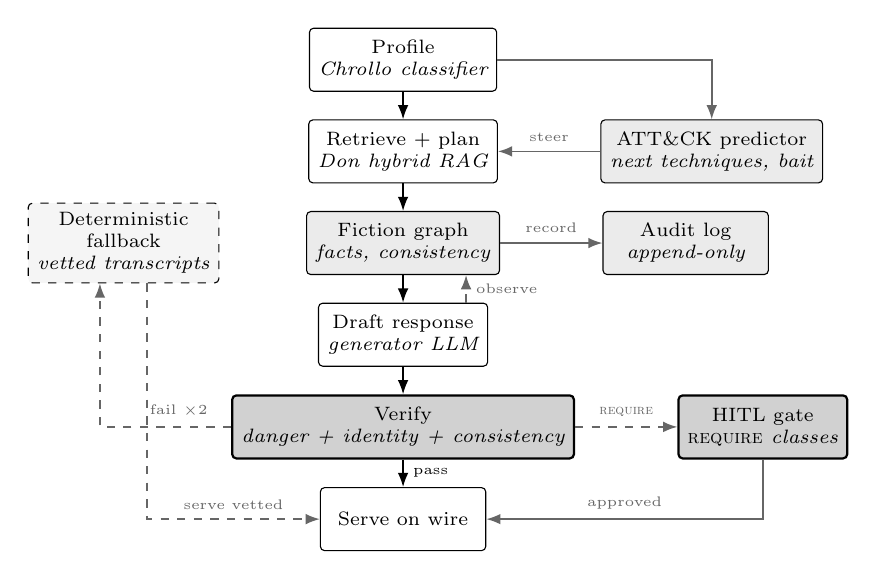
\begin{tikzpicture}[
  node distance=3.5mm and 5mm,
  stage/.style={draw, rounded corners=1.5pt, minimum height=8mm, minimum width=21mm, align=center, font=\scriptsize},
  store/.style={stage, fill=black!8},
  gate/.style={stage, fill=black!18, thick},
  fail/.style={draw, dashed, rounded corners=1.5pt, minimum height=8mm, align=center, font=\scriptsize, fill=black!4},
  arr/.style={-{Latex[length=1.8mm]}, semithick},
  farr/.style={arr, dashed, black!60}
]
% Main serving path (top to bottom)
\node[stage] (profile) {Profile\\ \scriptsize\itshape Chrollo classifier};
\node[stage, below=of profile] (retrieve) {Retrieve + plan\\ \scriptsize\itshape Don hybrid RAG};
\node[store, below=of retrieve] (graph) {Fiction graph\\ \scriptsize\itshape facts, consistency};
\node[stage, below=of graph] (draft) {Draft response\\ \scriptsize\itshape generator LLM};
\node[gate, below=of draft] (verify) {Verify\\ \scriptsize\itshape danger + identity + consistency};
\node[stage, below=of verify] (serve) {Serve on wire};

% Side stores
\node[store, right=13mm of retrieve] (mitre) {\attck predictor\\ \scriptsize\itshape next techniques, bait};
\node[store, right=13mm of graph] (audit) {Audit log\\ \scriptsize\itshape append-only};
\node[gate, right=13mm of verify] (hitl) {HITL gate\\ \scriptsize\itshape \textsc{require} classes};

% Failure path
\node[fail, left=11mm of graph] (fallback) {Deterministic\\ fallback\\ \scriptsize\itshape vetted transcripts};

% Main path arrows (vertical spine)
\draw[arr] (profile) -- (retrieve);
\draw[arr] (retrieve) -- (graph);
\draw[arr] (graph) -- (draft);
\draw[arr] (draft) -- (verify);
\draw[arr] (verify) -- (serve) node[midway, right, font=\tiny] {pass};

% Failure arrows: orthogonal, left corridor, offset anchors
\draw[farr] (verify.west) -| ([xshift=-3mm]fallback.south)
  node[pos=0.2, above, font=\tiny] {fail $\times$2};
\draw[farr] ([xshift=3mm]fallback.south) |- (serve.west)
  node[pos=0.75, above, font=\tiny] {serve vetted};

% Approval arrow: right corridor into serve.east
\draw[arr, black!60] (hitl.south) |- (serve.east)
  node[pos=0.75, above, font=\tiny] {approved};
\draw[farr] (verify.east) -- (hitl.west) node[midway, above, font=\tiny] {\textsc{require}};

% Feedback / context arrows: right gap, offset entry into graph.south
\draw[arr, black!60] (mitre) -- (retrieve) node[midway, above, font=\tiny] {steer};
\draw[arr, black!60] (profile.east) -| (mitre.north);
\draw[arr, black!60] (graph.east) -- (audit.west) node[midway, above, font=\tiny] {record};
\draw[farr] ([xshift=8mm]draft.north) -- ([xshift=8mm]graph.south)
  node[midway, right, font=\tiny] {observe};
\end{tikzpicture}

\caption{The verified deception loop. A session enters through the
behavioral classifier (Chrollo), which routes it to a per-class deception
policy. The retrieval engine (Don) grounds the policy in CTI; the fiction
graph binds every host fact; the generator drafts under the binding; the
verifier checks the draft against the graph before serving. Dashed paths
are failure paths: verification failure falls back to deterministic
transcripts, and content flagged \textsc{require} pauses at the
human-in-the-loop gate.}
\label{fig:architecture}
\end{figure*}

\subsection{Session Profiling: Behavioral Classification}
\label{sec:chrollo}
Each incoming session is first profiled by a lightweight behavioral
classifier (\emph{Chrollo}) that assigns the attacker to one of a small
set of classes (for example, automated scanner, credential stuffer,
hands-on-keyboard operator) using early-session signals: command cadence,
tool fingerprints, and target selection. The class determines which
deception policy the session receives: a scanner gets an attractive but
shallow surface, while an interactive operator is steered toward richer
bait. Profiling is kept cheap (a random forest over session features)
so that the expensive generative machinery is spent only on sessions
worth deceiving. Chrollo
satisfies the routing half of G1: \emph{who} the attacker is shapes
\emph{what} the deception tries to achieve.

\subsection{Grounded Planning: Retrieval-Augmented Deception}
\label{sec:don}
The retrieval engine (\emph{Don}) maintains a hybrid index over curated
CTI: dense embeddings for semantic recall and a lexical index for exact
indicator matching. Given the session profile and the attacker's observed
commands, Don retrieves the threat-intelligence context that the deception
plan should reflect: which techniques typically follow the ones the
attacker has already used, which bait artifacts are historically
effective
against this attacker class, and which indicators the plan should
be
seeded with. The planner converts retrieved intelligence into a
\emph{deception plan}: a set of facts to project, artifacts to expose, and
objectives to steer toward. G1 is measured here by construction; the
ablation in \S\ref{sec:evaluation} removes exactly this component.

\subsection{The Fiction Graph}
\label{sec:graph}
Every fact the honeypot projects about itself (hostname, kernel, listening
ports, installed databases, user accounts) is stored as a
subject--predicate--value triple in a per-session \emph{fiction graph}.
The graph is seeded from the host identity at session start and grows by
two mechanisms: \emph{declaration}, when the deception plan asserts a new
fact, and \emph{observation}, when a served response is scanned and any
host-like entities it emitted are extracted and recorded. Observation is
the mechanism that binds the LLM to the recorded state: whatever the generator said the
host is, the graph now remembers, and the next draft must agree with it.

A triple carries its source, and consistency is checked at the predicate
level: two declarations of the same predicate with different values raise
a contradiction, with normalization tuned to distinguish a genuine
conflict from a benign surface variant (a hostname is not contradicted by
its fully qualified form). When a contradiction is detected, the graph
records it and the verification node treats any draft resting on the
contradicted fact as unservable. The fiction graph is what turns G2 from
an aspiration into a data structure; the serving-time invariant below
states the consistency condition it enforces and its attacker-visible
scope.

\subsection{Verified Generation}
\label{sec:verify}
Generation is a draft, not a decision. The generator (a provider-hosted
LLM) receives the session context, the deception plan, a compact
serialization of the fiction graph (a \emph{fact block}), and the
steering context: the \attck techniques predicted to follow the
attacker's observed sequence, together with bait artifacts matched to
those techniques. The prediction uses the \attck tactic ordering to
propose the attacker's likely next moves (G1's steering half).

Before a draft reaches the wire it passes five checks:
\begin{enumerate}
\item \textbf{Danger scan.} A pattern gate rejects output that matches
credential-material, offensive-content, or real-secret signatures, with
one considered exemption: a single bare token that a real command would
print (the correct answer to \texttt{whoami} is one word) is not chatter.
\item \textbf{Identity pin.} Identity-revealing commands must answer from
the persona's pinned identity: a session classified as novice never
answers \texttt{whoami} with \texttt{root}, the hostname never changes
mid-session, and a root-prompting attempt is rejected rather than
obeyed. The C1 battery (\S\ref{sec:rq2}) carries a dedicated proof for
this check.
\item \textbf{Consistency check.} Host-like entities in the draft are
observed into the fiction graph; a draft that introduces a contradictory
fact is rejected with the contradiction recorded.
\item \textbf{Supported-claim check.} On a declared command surface whose
real-Linux output is deterministic given the pinned identity (identity
queries, kernel and OS facts, echo, uptime and date shapes, the
OS-release file), the draft must \emph{contain} the correct answer:
hedging, echoing the query back, or omitting the answer is a rejection,
not a pass. Outside the declared surface the check is silent, so recall
on open-ended attacker behavior is untouched by this closed surface.
\item \textbf{Terminal sanity.} Shell-shaped responses that answer a
command with sentence-like chatter rather than command output are
rejected as degenerate.
\end{enumerate}
A draft that fails any check is retried once with the violation fed back;
a second failure triggers fallback. The checks were selected by one
criterion: each must be a \emph{decision procedure} over the draft,
decidable, cheap, and deterministic, because a verifier that itself calls
a model would only relocate the trust problem it exists to solve. What
verification deliberately does not certify is quality. A draft can pass
all five checks and still be unpersuasive; plausibility is not
decidable, and the paper does not pretend otherwise. The division of
labor is the point: the loop's machinery enforces the three properties
of the three safety constraints machine-checkably, and the consensus study of
\S\ref{sec:rq3} assesses the deception quality that only evaluation can
measure. This is the mechanism behind the zero-unverified-serves claim
evaluated in \S\ref{sec:evaluation};
The serving sequence above gives the full loop, and its fallback arm is
what carries G4 while its
\textsc{Require} branch carries G3.

\subsection{Cross-Session Host Fiction}
\label{sec:hostfiction}
The per-session fiction buys bounded blast radius
at a measured price: a returning attacker is shown a fresh world, and
none of the session verifier's checks can see drift \emph{between}
sessions. The host-fiction layer closes exactly that gap without
widening the blast radius. It is host-keyed rather than session-keyed:
at an attacker's first contact with a host, its identity is pinned and
provisioned into every consumer --- the persona prompt is rebuilt from
the pinned identity (removing a class of contradictory-instruction
failures where prompt and verifier disagreed), the session graph is
seeded authoritatively for verification, and the fallback template
inherits the same identity. Facts observed in a session are promoted to
the host store only when they passed verification (fail-closed: an
unverified session never binds a host fact), and every subsequent
session against the same host is cross-checked against the promoted
set by a session-verifier wrapper that rejects on cross-session
contradiction. Reconnect policies are configurable: a returning
connection can share the pinned graph outright, or start a promoted
session whose facts are cross-checked against the host.

The layer is measured, not merely present. On identical deterministic
drift scenarios (reconnect drift, beyond-identity drift, cross-skill
host swap, simultaneous contradiction, repetition controls), the
session-scoped verifier alone catches 1 of 4 cross-session drift drafts;
both host-fiction policies catch 4 of 4 with 0 of 7 benign re-query
false rejections (\path{cross_session_consistency_bench.json}). The
three misses of the session-scoped baseline are invisible to it by
construction --- facts asserted in a previous session simply are not in
current-session state --- and per-skill identities name different hosts,
so a reclassified returning attacker would otherwise be shown a
different machine. On benign traffic the layer is free: paired over the
full 218-query workload, store-on versus store-off serves byte-identical
strings on every row (paired per-row delta exactly $0.0000$;
\path{external_baseline_hostfiction_comparison.json}), so cross-session
consistency is added at zero quality cost on the evaluated surface.

\subsection{Human-in-the-Loop Gate}
\label{sec:hitl}
Content classes whose compromise value is high (deployed credentials,
for instance) are marked \textsc{require} in the deception policy. When a
response would serve such content, the loop pauses and the decision is
surfaced to the operator through an audit interface that records the
context, the draft, and the decision. Every gate decision is persisted to
an append-only audit log, which \S\ref{sec:evaluation} uses as a
correctness and governance record.
The gate encodes a governance position: the system may \emph{draft}
deception, but a human decides when the deception includes trap
material (G3). The gate exists for the operator's stake, not the
attacker's: canary bait is safe to serve by construction, but it is
still an active measure whose use an operator may be required to
authorize; the audit record of that authorization leaves the system
defensible after the fact. The require-level branch is also where the
credential-deployment decisions in the benchmark trail
(Appendix~\ref{app:audit}) were made.

\subsection{Deterministic Fallback}
\label{sec:fallback}
Every scenario class has a vetted deterministic transcript: hand-written,
fiction-consistent bait and response templates (credential hunts, service
enumerations, exfiltration decoys) whose secrets are registered canaries.
When generation fails, the provider times out, verification rejects twice,
or the model refuses the persona, the loop serves the deterministic
transcript for the scenario instead. The fallback is not an admission of
defeat; it is the safety floor that makes the LLM path safe to enable.
The A5 ablation checks that the system is \emph{equivalent} through the
fallback path, and the design of the canary registration is what allows
the consensus study to distinguish deployed bait from accidental leaks.

Session state beyond identity facts replays the same discipline. A
filesystem ledger records the bytes served for every read command and
replays them verbatim when the same path is read again; time-varying
ambient content (process identifiers, timestamps, clock outputs) is not
stored but generated by hashing a per-session seed through a template,
so re-reads are identical within a session while sessions differ
plausibly from one another, and a mutating command invalidates the
affected entries so subsequent reads reflect the mutation. This ledger,
not the generative path, is what the byte-identical replay component of
the C1 result (\S\ref{sec:rq2}) exercises: determinism on re-query is a
property of how session state is stored and replayed, and the design
keeps it decoupled from generation.
The fallback also carries a hidden load: it defines the system's floor
under failure. Because the fallback serves the same fiction the generator
would have, an attacker cannot distinguish a degraded session from a
healthy one by content alone; the availability
property of G4 thereby becomes a deception property, not merely a reliability one.
What the fallback gives up is the generator's adaptivity: a fallback
session answers within its scenario's script and steers no further,
which is the correct trade only because the loop treats it as a floor
beneath the LLM path rather than the path itself.

\subsection{A Session Through the Loop}
\label{sec:example}
A single ground-truth session shows the machinery cooperating. The
attacker opens with a cloud-credential probe:
\begin{quote}\small
\texttt{curl~}\path{http://169.254.169.254/latest/meta-data/}
\end{quote}
Chrollo classifies the cadence and target as an intermediate operator
hunting instance credentials; Don retrieves the IMDS abuse pattern and
maps it to \attck T1552.005, and the predictor ranks metadata-API
credential theft as the attacker's active objective. The deception plan
accordingly projects an EC2-shaped identity, and the generator drafts the
IMDSv2 flow: token PUT, role listing, and a credential document whose
access key is a registered canary in the ASIA temporary-key shape. The
verifier observes the draft's host facts (instance id, role name, region
mapping) into the fiction graph, confirms the document is consistent with
every prior turn, and passes it; the danger scan passes because the
key material is canary-registered rather than real. The draft is one of
the content classes marked \textsc{require}, so the loop pauses at the
HITL gate, records the context and the decision in the append-only audit
log, and serves the artifact only on operator approval. The transcript
the attacker sees is an ordinary credential dump; the record the operator
sees is the full decision chain, and any later appearance of the canary
key in outbound traffic is attributable to this session by construction.

The loop's failure path deserves an equally concrete telling, because
the design's central claim is that it is safe, not merely present. The
same session, one turn later, asks the honeypot to retrieve a file. The
classifier and planner do their work unchanged, and the generator
drafts a directory listing -- but the draft invents a second network
interface with an IP address on a subnet the plan never advertised, and
the seed identity pins this host to one interface. The consistency
check observes the draft's host facts into the fiction graph, the
closure flags the conflict against the pinned interface, and the draft
is rejected with the contradiction recorded; nothing was served, so
nothing entered the graph and nothing reached the attacker. The retry
receives the violation as feedback and drafts again -- and this time
commits the subtler error of quoting a kernel build timestamp that
contradicts the one printed in the session's first turn. Rejected
again. On the second failure the loop stops trusting the generator for
this turn entirely and serves the scenario's vetted deterministic
transcript: same fiction, same canary discipline, no adaptation, and no
visible seam -- the attacker's next command meets a prompt line exactly
as it would have after a verified serve. What the operator's audit log
records is the difference: two verifier rejections with their
contradictions, one fallback serve, and a session whose fiction state
is byte-for-byte what it would have been had the generator never been
consulted. The transcript the attacker sees and the one a healthy
session would have shown are indistinguishable by content; only the
audit trail knows the generator was dropped.

\subsection{Loop Orchestration}
\label{sec:orchestration}
The loop is compiled as an explicit state machine: profile, retrieve,
plan, draft, verify, serve (or fallback), with per-node state persisted so
that a paused session (at the HITL gate, for instance) resumes exactly
where it stopped. A linear fallback path mirrors the same nodes without
the graph machinery, and the A5 ablation confirms the two paths are
behaviorally equivalent when the graph adds no information. Orchestration
makes the loop auditable end to end: every session has a recorded
path through the nodes, which the stability analysis of
\S\ref{sec:evaluation} replays.

\section{Related Work}
\label{sec:related}

\subsection{Honeypots and Cyber Deception}

Surveys of large language models in security \cite{wang2024} and of cyber
deception specifically \cite{lopez2024} frame the opportunity and its open
questions. Honeypots have been studied as instrumentation for two decades
\cite{spitzner2002}, and their engineering trade-offs---visibility,
fidelity, and the operational cost of interaction---remain open
\cite{sokol2017}. Adaptive deception work formalizes the
defender's decision to engage, treating attacker intent as something to
infer and modulate, through factored interactive POMDPs
\cite{shinde2020}, engagement--yield models
\cite{bera2024}, and behavioral partitioning under cognitive load
\cite{liska2024}. Deception has also been embedded in higher-fidelity
simulation and emulation targets \cite{kouremetis2024}. We adopt as our
starting point the gap that deception-framework surveys identify in deployed
systems: that they neither ground responses in live threat intelligence
nor differentiate behavior across attacker classes \cite{lopez2024}. Our
contribution is orthogonal to that taxonomy. We do not propose a new
deception policy; we constrain what a generative policy is allowed to serve.

\subsection{Generative Honeypots}

The closest prior art puts a language model inside the deception endpoint.
LLM-in-the-shell honeypots make the model answer as a live machine
\cite{valeros2024}; LLM agent honeypots instead monitor autonomous AI
attackers in the wild \cite{reworr2024}; and recent systems extend
generative deception to industrial protocols and physical-process emulation
\cite{vasilatos2025llmpot}, coordinated IoT deception
\cite{guan2025cpds}, and directory services
\cite{jimenez2025}. Analysis pipelines over collected honeypot and
incident data apply generative or learned models after the fact, for attack
classification and reporting \cite{lanka2024,simoni2024,blefari2025},
structured CTI mapping \cite{orbinato2022}, and attack investigation
\cite{alsaheel2021}. In all of these the model
output is the product. None of them states a serving contract for it: no
fixed fiction to be consistent with, no deterministic gate that can refuse
a draft, and no vetted answer to fall back to when the provider refuses or
times out. That contract, and the ladder analysis that prices it, is what
this paper adds; the generative mechanisms themselves are borrowed.

\subsection{Runtime Enforcement and Red-Teaming of LLM Applications}

The verifier is the closest analogue in prior art, and the analogy is
deliberate. AgentSpec provides customizable runtime enforcement for LLM
agents \cite{wang2026agentspec}; prompt-injection defences that constrain
decoding or shape preference rather than trusting a probability are
proposed in \cite{chen2025struq} and \cite{chen2025secalign}; the injection
threat they answer is formalized in \cite{greshake2023} and measured by
AgentDojo \cite{debenedetti2024agentdojo}; the wider surface of tool-bearing
agents adds cross-tool harvesting and pollution \cite{li2026dissonances};
model-written and
model-red-teamed evaluation is standard practice
\cite{ganguli2022,perez2022,bai2022,christiano2017}. Our design follows
that literature's premise that assurance must live outside the model. What
differs is the asset being protected. A guardrail protects the assistant's
user from the model's output; this gate protects the attacker's belief from
the fiction's, so the failure of interest is a fluent, self-consistent,
on-script response that is nonetheless wrong for the deception state, and
the mitigation is a deterministic fallback to vetted content rather than a
refusal.

\subsection{Retrieval Grounding, and the Attacks We Do Not Yet Resist}

Retrieval grounding supplies the targeting rung
\cite{lewis2020}, and retrieval for threat intelligence is well populated:
technique extraction and TTP analysis \cite{fayyazi2023,lekssays2025},
knowledge-graph constructions \cite{gao2025,jeon2024,belmahjoub2025},
knowledge-graph index families \cite{malkov2018} that we price against
sparse retrieval, investigation and response assistants
\cite{rajapaksha2024,paul2025,qiao2025,liu2025}, and the \attck{}
grounding question itself \cite{roy2023,alsada2024,noureddine2020}. The
security of that retrieval layer is a separate and active literature:
benchmarking and vulnerability identification \cite{xue2024,liang2025},
adversarial threat vectors and mitigations for RAG systems
\cite{ward2025}, knowledge corruption \cite{zou2025poisonedrag,chaudhari2024},
retrieval jamming \cite{shafran2024}, in-place and indirect poisoning
evaluation \cite{malladi2026ripeii}, poisoning-aware ranking for CTI
pipelines \cite{jia2025}, and responsibility attribution for poisoned
knowledge \cite{zhang2026ragorigin}. We adopt that literature's threat
model as out of scope for demonstrated results: this paper evaluates no
retrieval poisoning and no injection defence, and
Section~\ref{sec:threat-model} records that as a gap rather than a
result. We price that scoping rather than hide it. The retrieval layer sits
inside the threat surface this literature has already mapped, so a deployment
that inherits it inherits those attacks, and the grounding rung's measured
benefit of $+0.154$ is a benefit under an undefended retrieval layer. Closing
that is a prerequisite for treating the grounding result as a security
contribution rather than a capability one.

\subsection{Deception Quality Judged by Machines}

Because no human study is claimed, the relevant prior art is LLM-as-judge
methodology: MT-Bench and Chatbot Arena for judge agreement
\cite{zheng2024}, JudgeBench for judge reliability \cite{tan2025judgebench},
and optimization-based attacks against the judge itself
\cite{shi2024judgedeceiver}. The third of these is the reason our quality
section reports within-model consistency with an audited judge rather than
presenting a realism score as validated.

\subsection{Position}

We are not the first to build a language model into a honeypot, and we do
not claim a new deception policy, a new retrieval stack, or a new
enforcement primitive. The contribution is the composition: a fixed
deception state, a deterministic gate that disposes against it, a vetted
floor beneath it, and an explicit ladder analysis that prices each
intelligence mechanism against its cheapest certifiable competitor---then
removes the rungs that do not pay.
\section{Evaluation}
\label{sec:evaluation}

% Results figures, rendered from the persisted artifacts:
% bootstrap_ci.json (suite means and 95% CIs), stability_run1_vs_run2.json (run pairs).
% Values resolve through figures/generated_values.tex, which scripts/gen_sp_figures.py
% writes from those artifacts; run `python scripts/gen_sp_figures.py --check` to prove
% this figure still agrees with them.
% Layout discipline: the top panel shows point estimates + intervals only
% (no filled bars under the whiskers), the bottom panel's legend lives
% below the axis (never over the bars), and both panels share the same
% value range so the stacked scales read as one.
% GENERATED by scripts/gen_sp_figures.py -- do not edit by hand.
% Every plotted number in the S&P figures resolves through this file, so a
% figure cannot silently disagree with the artifact it claims to show.
% Regenerate:  python scripts/gen_sp_figures.py
% Verify:      python scripts/gen_sp_figures.py --check
% Sources:
%   results/bootstrap_ci.json
%   results/stability_run1_vs_run2.json
%   results/b4_baseline_zodiac_20260922.json
%   results/model_quality/chrollo_calibration.json
%   results/sp2027_rescue/behavior_trajectory_benchmark.json

\def\RaginLiveTechnique{0.9598}
\def\RaginLiveTechniqueErrLo{0.0122}
\def\RaginLiveTechniqueErrHi{0.0122}
\def\RaginLiveActor{0.8500}
\def\RaginLiveActorErrLo{0.0000}
\def\RaginLiveActorErrHi{0.0000}
\def\RaginLivePersona{0.7325}
\def\RaginLivePersonaErrLo{0.0587}
\def\RaginLivePersonaErrHi{0.0558}
\def\RaginLiveComposite{0.8796}
\def\RaginLiveCompositeErrLo{0.0224}
\def\RaginLiveCompositeErrHi{0.0204}
\def\RaginLivePersonaRunTwo{0.7504}
\def\RaginLiveCompositeRunTwo{0.8845}
\def\RaginPersonaRunDelta{0.018}
\def\RaginTechDelta{0.317}
\def\RaginTechDeltaLo{0.162}
\def\RaginTechDeltaHi{0.480}
\def\RaginActorDelta{0.140}
\def\RaginActorDeltaLo{0.083}
\def\RaginActorDeltaHi{0.197}
\def\RaginPersonaNullDelta{0.005}
\def\RaginPersonaNullDeltaLo{-0.047}
\def\RaginPersonaNullDeltaHi{0.057}
\def\RaginOverallDelta{0.154}
\def\RaginOverallDeltaLo{0.092}
\def\RaginOverallDeltaHi{0.221}
\def\RaginGroundingTtpCount{35}
\def\RaginNoGroundingTtpCount{0}
\def\RaginRoutingBefore{0.8875}
\def\RaginRoutingAfter{0.955}

\begin{figure}[t]
\centering
\begin{tikzpicture}
\begin{axis}[
  name=ax1,
  width=0.96\linewidth,
  height=4.9cm,
  xmin=0.55, xmax=1.02,
  y axis line style={draw=none},
  axis x line*=bottom,
  axis y line*=left,
  ytick=data,
  yticklabels={Composite,Persona,CTI actor$^{\dagger}$,CTI technique},
  y dir=reverse,
  xlabel={score (95\% CI)},
  xlabel style={font=\footnotesize},
  tick label style={font=\footnotesize},
  enlarge y limits=0.6,
  grid=major,
  grid style={black!10},
  clip=false
]
% point estimates and bootstrap 95% CIs from bootstrap_ci.json;
% only marks + intervals: no bars beneath the whiskers
\addplot+[only marks, mark=|, mark size=3.4, mark options={thick,black},
  error bars/.cd, x dir=both, x explicit] coordinates {
  (\RaginLiveTechnique,3) +- (\RaginLiveTechniqueErrLo,\RaginLiveTechniqueErrHi)
  (\RaginLiveActor,2) +- (\RaginLiveActorErrLo,\RaginLiveActorErrHi)
  (\RaginLivePersona,1) +- (\RaginLivePersonaErrLo,\RaginLivePersonaErrHi)
  (\RaginLiveComposite,0) +- (\RaginLiveCompositeErrLo,\RaginLiveCompositeErrHi)
};
% run-2 overlay: open markers (point estimates from stability_run1_vs_run2.json;
% per-suite CIs were not computed for run 2, so none are drawn)
\addplot+[only marks, mark=o, mark size=1.9, mark options={semithick,black!60}] coordinates {
  (\RaginLiveTechnique,3)
  (\RaginLiveActor,2)
  (\RaginLivePersonaRunTwo,1)
  (\RaginLiveCompositeRunTwo,0)
};
\end{axis}
\end{tikzpicture}

\vspace{2mm}

\begin{tikzpicture}
\begin{axis}[
  name=ax2,
  width=0.96\linewidth,
  height=4.9cm,
  ybar=1.5pt,
  bar width=9pt,
  ymin=0.55, ymax=1.0,
  symbolic x coords={CTI technique,CTI actor,Persona,Composite},
  xtick=data,
  ylabel={mean score},
  ylabel style={font=\footnotesize},
  tick label style={font=\footnotesize},
  ymajorgrids,
  grid style={black!10},
  enlarge x limits=0.25,
  legend style={font=\scriptsize, at={(0.5,-0.16)}, anchor=north, legend columns=2, draw=none, fill=none},
  legend cell align={left},
]
% run 1 vs run 2 from stability_run1_vs_run2.json
\addplot+[black!35, fill=black!35] coordinates {
  (CTI technique,\RaginLiveTechnique) (CTI actor,\RaginLiveActor) (Persona,\RaginLivePersona) (Composite,\RaginLiveComposite)
};
\addplot+[black!70, fill=black!70, pattern=north east lines] coordinates {
  (CTI technique,\RaginLiveTechnique) (CTI actor,\RaginLiveActor) (Persona,\RaginLivePersonaRunTwo) (Composite,\RaginLiveCompositeRunTwo)
};
\legend{run 1, run 2}
\end{axis}
\end{tikzpicture}
\caption{Live-campaign results from the persisted artifacts (identical
deterministic-strata bars across runs are the finding, not a plotting
error). All four plotted values are the \emph{both-channel} operational
score of Table~\ref{tab:live}, which fuses the served-text and CTI-analysis
channels; they are not served-quality results, and the echo-guarded bounds
for the same rows are 0.479 technique and 0.243 actor.
\emph{Top:}
suite means with bootstrap 95\% confidence intervals; open markers mark
the independent second run's point estimates, and the actor interval is
degenerate ($^{\dagger}$) because the actor rubric assigns the same
score to every row, so uncertainty is carried by the Wilson pass-rate
interval instead (Table~\ref{tab:live}). \emph{Bottom:} two independent
218-query campaigns; the deterministic CTI strata replicate exactly and
only the LLM-judged persona stratum moves, by $+\RaginPersonaRunDelta$.}
\label{fig:results}
\end{figure}


We evaluate the loop as a serving system, separating what the attacker
receives (the \emph{served-text} channel) from what the retrieval pipeline
identifies for the operator (the \emph{CTI-analysis} channel). The latter is
never served. All headline results are backed by persisted JSON or JSONL
artifacts. Paired grounding differences use a 10,000-resample percentile
bootstrap over scenario-level differences. The induced-draft battery instead
resamples whole \emph{cases} (cluster bootstrap, 10,000 iterations, unit =
case), because the repeats inside a case share one scenario and are not
independent; its intervals are therefore wider than the draft-level binomial
intervals they replace, and the draft-level ones are not used. The
deterministic suites carry exactly one draft per case, so clustering is
vacuous there and their intervals are binomial over cases.

\subsection{Setup and Grounding}
\label{sec:setup}
The archived runs execute against a 2-vCPU, ${\sim}4$-GB single-host
deployment; the evaluation harness runs on a separate workstation and shares
no state with the deployed stack. The fixed
workload contains 123 CTI-technique queries, 35 CTI-actor queries, and 60
persona sessions. The generator and judge use different model families from
one free-tier provider; catalog drift, quota exhaustion, gateway outages, and
alignment refusals are absorbed by the deterministic floor. Fresh
provider-backed reruns are currently unavailable. The paired grounding
experiment runs 30 scenarios in each of the technique, actor, and persona
strata with identical prompts and retrieval removed only in the control arm.
Because that design is balanced across strata while the live workload is not,
the ablation estimates a balanced-stratum mean difference rather than the
deployment-weighted composite of Table~\ref{tab:live}; the two are not the
same estimand, and no correction is applied across the three strata and the
pooled row because each interval is already far from its null.

Table~\ref{tab:provenance} records which generator produced which surface.
The surfaces were not produced by one model, so results are not compared
across them; the version-of-record campaign predates the model pin and its
generator was not logged.

\begin{table*}[t]
\centering
\caption{Generator provenance per measured surface. The campaign, the ladder,
and the scorer audit were produced by three different generators; no number is
compared across rows.}
\label{tab:provenance}
\scriptsize
\setlength{\tabcolsep}{5pt}
\begin{tabular}{p{0.33\textwidth}>{\raggedright\arraybackslash}p{0.60\textwidth}}
\toprule
Surface & Generator / gateway \\
\midrule
Paired grounding ablation (Table~\ref{tab:b4})
  & not logged (pre-pin gateway default) \\
Version-of-record campaign (Table~\ref{tab:live})
  & not logged (pre-pin gateway default) \\
Same-model ladder (Table~\ref{tab:baseline-served-text})
  & \texttt{deepseek-v4-flash-free} on \texttt{api.apmix.ai} \\
Scorer-validity audit corpus (\S\ref{sec:scorer-audit})
  & gateway default (\texttt{glm-5.3-flash-free}) \\
Induced-draft battery (Table~\ref{tab:verifier-cross-family})
  & \texttt{space-bunny-free}, \texttt{deepseek-v4-flash-free} on
    \texttt{api.apmix.ai}; \texttt{llama-3.3-70b-instruct} on
    \texttt{openrouter.ai} \\
Deception-quality judge (\S\ref{sec:rq3})
  & one judge model, same provider as the generator \\
\bottomrule
\end{tabular}
\end{table*}

\begin{table}[t]
\centering
\caption{Paired grounding ablation: 90 matched scenario pairs. Scores are
the declared analysis-channel composite; channel attribution follows the
recorded scorer configuration and measurement lineage, as the archived
artifact carries no channel field. CIs are paired bootstrap intervals.
The archived artifact pairs by scenario name; new reruns must persist canonical
scenario IDs and manifest hashes.}
\label{tab:b4}
\scriptsize
\setlength{\tabcolsep}{3.5pt}
\begin{tabular}{lccc}
\toprule
Suite & RAG & No-RAG & Difference (95\% CI) \\
\midrule
Technique & 0.950 & 0.633 & $+0.317$ $[+0.162,+0.480]$ \\
Actor & 0.850 & 0.710 & $+0.140$ $[+0.083,+0.197]$ \\
Persona & 0.833 & 0.828 & $+0.005$ $[-0.047,+0.057]$ \\
\midrule
Overall & & & $+0.154$ $[+0.092,+0.221]$ \\
\bottomrule
\end{tabular}
\end{table}

% Paired grounding effect (RAG minus No-RAG) per suite with 95% bootstrap
% CIs, from b4_baseline_zodiac_20260922.json (the same numbers as
% Table~tab:b4). Filled markers: intervals excluding zero. Open marker:
% the persona stratum, whose interval straddles zero exactly as the
% architecture predicts. Compiled statically; no results directory needed.
% GENERATED by scripts/gen_sp_figures.py -- do not edit by hand.
% Every plotted number in the S&P figures resolves through this file, so a
% figure cannot silently disagree with the artifact it claims to show.
% Regenerate:  python scripts/gen_sp_figures.py
% Verify:      python scripts/gen_sp_figures.py --check
% Sources:
%   results/bootstrap_ci.json
%   results/stability_run1_vs_run2.json
%   results/b4_baseline_zodiac_20260922.json
%   results/model_quality/chrollo_calibration.json
%   results/sp2027_rescue/behavior_trajectory_benchmark.json

\def\RaginLiveTechnique{0.9598}
\def\RaginLiveTechniqueErrLo{0.0122}
\def\RaginLiveTechniqueErrHi{0.0122}
\def\RaginLiveActor{0.8500}
\def\RaginLiveActorErrLo{0.0000}
\def\RaginLiveActorErrHi{0.0000}
\def\RaginLivePersona{0.7325}
\def\RaginLivePersonaErrLo{0.0587}
\def\RaginLivePersonaErrHi{0.0558}
\def\RaginLiveComposite{0.8796}
\def\RaginLiveCompositeErrLo{0.0224}
\def\RaginLiveCompositeErrHi{0.0204}
\def\RaginLivePersonaRunTwo{0.7504}
\def\RaginLiveCompositeRunTwo{0.8845}
\def\RaginPersonaRunDelta{0.018}
\def\RaginTechDelta{0.317}
\def\RaginTechDeltaLo{0.162}
\def\RaginTechDeltaHi{0.480}
\def\RaginActorDelta{0.140}
\def\RaginActorDeltaLo{0.083}
\def\RaginActorDeltaHi{0.197}
\def\RaginPersonaNullDelta{0.005}
\def\RaginPersonaNullDeltaLo{-0.047}
\def\RaginPersonaNullDeltaHi{0.057}
\def\RaginOverallDelta{0.154}
\def\RaginOverallDeltaLo{0.092}
\def\RaginOverallDeltaHi{0.221}
\def\RaginGroundingTtpCount{35}
\def\RaginNoGroundingTtpCount{0}
\def\RaginRoutingBefore{0.8875}
\def\RaginRoutingAfter{0.955}

\begin{figure}[t]
\centering
\begin{tikzpicture}[
  font=\scriptsize,
  dot/.style={circle, fill=black, inner sep=1.5pt},
  nul/.style={circle, draw=black, fill=white, inner sep=1.5pt, thick},
  arr/.style={-{Latex[length=1.6mm]}, semithick, black!55}
]
  % zero reference
  \draw[black!45] (0,0.5) -- (0,-3.2);
  \node[font=\tiny, text=black!60, anchor=east] at (-0.05,0.5) {$\Delta=0$};

  % CTI technique: +0.317 [+0.162, +0.480]
  \node[anchor=east] at (-0.25,0) {CTI technique};
  \draw[black!70] (1.62,0) -- (4.80,0);
  \draw[black!70] (1.62,-0.13) -- (1.62,0.13);
  \draw[black!70] (4.80,-0.13) -- (4.80,0.13);
  \node[dot] at (3.17,0) {};

  % CTI actor: +0.140 [+0.083, +0.197]
  \node[anchor=east] at (-0.25,-0.95) {CTI actor};
  \draw[black!70] (0.83,-0.95) -- (1.97,-0.95);
  \draw[black!70] (0.83,-1.08) -- (0.83,-0.82);
  \draw[black!70] (1.97,-1.08) -- (1.97,-0.82);
  \node[dot] at (1.40,-0.95) {};

  % Persona (predicted null): +0.005 [-0.047, +0.057]
  \node[anchor=east] at (-0.25,-1.9) {Persona};
  \draw[black!70] (-0.47,-1.9) -- (0.57,-1.9);
  \draw[black!70] (-0.47,-2.03) -- (-0.47,-1.77);
  \draw[black!70] (0.57,-2.03) -- (0.57,-1.77);
  \node[nul] at (0.05,-1.9) {};

  % Overall
  \draw[black!25, dashed] (-0.25,-2.5) -- (5.0,-2.5);
  \node[anchor=east] at (-0.25,-3.0) {Overall (90 pairs)};
  \draw[black!70] (0.92,-3.0) -- (2.21,-3.0);
  \draw[black!70] (0.92,-3.13) -- (0.92,-2.87);
  \draw[black!70] (2.21,-3.13) -- (2.21,-2.87);
  \node[dot] at (1.54,-3.0) {};

  % axis
  \draw[arr] (0,-3.65) -- (5.1,-3.65);
  \foreach \x/\l in {0/0, 1/{+0.1}, 2/{+0.2}, 3/{+0.3}, 4/{+0.4}} {
    \draw[black!55] (\x,-3.58) -- (\x,-3.72)
        node[below, font=\tiny, text=black!60] {\l};
  }
\end{tikzpicture}
\caption{Paired grounding differential (RAG $-$ No-RAG) per suite with
95\% bootstrap CIs over 90 scenario pairs (numbers in
Table~\ref{tab:b4}). Filled markers: intervals excluding zero -- $+\RaginTechDelta$
on technique detection and $+\RaginActorDelta$ on actor attribution. The open
marker is the persona stratum, whose interval straddles zero exactly as
the architecture predicts: host believability is produced by the
deception engine and the fiction graph, not by threat-intelligence
retrieval. The mechanism behind the technique effect is starker than
the mean: the grounded arm yields \RaginGroundingTtpCount{} TTP detections spanning 21 distinct
techniques, while the ungrounded arm yields none.}
\label{fig:grounding}
\end{figure}


The analysis channel detects 35 TTPs spanning 21 techniques versus zero
without retrieval, while persona realism remains unchanged. The null is informative:
host believability is produced by the fiction graph and deception engine,
whereas CTI intelligence is the retrieval-dependent capability. The full
grounded campaign records 132 detections spanning 67 unique techniques.

\subsection{Serving Safety and Induced Failures}
\label{sec:rq2}
The live workload records zero contradictions across 45 targeted re-queries,
zero pinned-identity violations, and zero serves after a failed verifier
verdict. In the 218-query campaign, 218 sessions engage and 218 persona
assignments are correct; the declared both-channel composite is 0.880, which
Table~\ref{tab:live} reports beside its echo-guarded bound rather than as a
standalone capability score.

Serve-path provenance is taken from the per-serve labels the pipeline stamps,
not from response time: the archived tally records 216 of 218 responses as
\texttt{GENERATED\_VERIFIED} and 2 as \texttt{FALLBACK\_VERIFIED}, with no
serve labeled as a fail-safe substitution. A later scorer-validity audit
found that gateway-outage and template-anchored serves had carried no marker
in that tally and were counted as verified generation; they are now stamped
\texttt{TEMPLATE\_FALLBACK\_VERIFIED}, and roughly one hundred rows on the
CTI surface serve template-echoed text. A latency-based cross-check that
classifies any turn faster than $4\,\mathrm{s}$ as vetted deterministic
content estimates an $88.1/11.9$ split --- a lower bound on the deterministic
share rather than an audited count. One disclosure bounds the
zero-contradiction claim: 11.9\% of serves are estimated deterministic-path,
so some of the 45 re-queries may be template serves for which consistency is
a property of the vetted library rather than graph-enforced generation. A
serve-path-stamped re-run remains future work; the zero-contradiction result
itself is unaffected, since both serve paths are verified or vetted by
construction.

\begin{table}[t]
\centering
\caption{Version-of-record 218-row campaign. Column~3 is the declared
\emph{both-channel} operational score, which fuses the served-text and
CTI-analysis channels and therefore is not a served-quality result. Column~4
is the echo-guarded lower bound computed on these same archived rows, where
template-echo rows are zeroed and the remainder keeps its both-channel score;
because the stored responses are truncated previews, column~4 is a lower
bound and not the guarded served-text mean.}
\label{tab:live}
\scriptsize
\setlength{\tabcolsep}{4pt}
\begin{tabular}{lrrr}
\toprule
Suite & $n$ & Both-channel & Guarded LB \\
\midrule
Technique & 123 & 0.960 & 0.479 \\
Actor & 35 & 0.850 & 0.243 \\
Persona & 60 & 0.733 & 0.733 \\
\midrule
Composite & 218 & 0.880 & 0.511 \\
\bottomrule
\end{tabular}
\end{table}

\begin{table}[t]
\centering
\caption{Verifier stress test after the P1 extraction fixes. Live rows are
authored drafts, not served sessions; the llama row includes 48 disclosed
substitute-author fills. Intervals are 95\% cluster bootstraps that resample
cases (89, 80, and 94 cases; 105 for the deterministic suite, which carries one
draft per case). Bootstrapping cases rather than drafts widens the llama
precision interval from $[.869,.947]$ to $[.858,.962]$.}
\label{tab:verifier-cross-family}
\scriptsize
\setlength{\tabcolsep}{2.5pt}
\begin{tabular}{lrrrrr}
\toprule
Author & Drafts & P & 95\% CI & R & 95\% CI \\
\midrule
space-bunny-free & 261 & 1.000 & $[1.000,1.000]$ & 0.959 & $[.926,.985]$ \\
deepseek-v4-flash-free & 236 & 1.000 & $[1.000,1.000]$ & 0.983 & $[.961,1.000]$ \\
llama-3.3-70b & 281 & 0.916 & $[.858,.962]$ & 0.898 & $[.848,.943]$ \\
\midrule
Pooled (778 drafts) & 778 & 0.970 & $[.949,.987]$ & 0.944 & $[.922,.965]$ \\
Canonical deterministic & 105 & 1.000 & -- & 1.000 & -- \\
\bottomrule
\end{tabular}
\end{table}

The clean workload tests the deployed serving invariant, not sensitivity to
bad drafts. The canonical 105-case suite has 78 reject and 27 pass cases and
achieves perfect precision and recall on danger, identity, consistency, and
degenerate checks. The cross-family matrix induces failures and exposes the
real boundary: post-fix recall is 0.898--0.983 and precision is
0.916--1.000. Residual errors concentrate in author-side identity drift and
model-specific tell vocabulary. Thus the paper claims fail-closed serving,
not universal semantic coverage.

\paragraph{What the gate prevented.}
The clean campaign does not exercise the gate. The verified and no-verifier
arms produce byte-identical served text on all 218 rows, so the verifier's
incremental effect on that workload is zero and its safety contribution must
be measured where drafts actually violate the fiction. Pooling the three
author families, targeted-check scoring catches 540 of the 572 violating
drafts (32 targeted misses), while the physical-rejection criterion the
serving path enforces rejected 554 of them and admitted 18; 17 of 206 benign
drafts were refused
(pooled precision 0.970 $[.949,.987]$, recall 0.944 $[.922,.965]$, cluster
bootstraps that resample cases within each author family). The one fully
attributed family (llama-3.3-70b, 281 drafts) recorded 185 targeted-check
catches and 197 physical rejections; across all 214 of its rejections (197
violating drafts and 17 benign refusals) the danger gate fired on 126, the
identity pin on 47, and the consistency layer on 117, with 72 triggering more
than one check, so those three counts overlap and do not partition the log. Each rejected violating draft
was a response that would otherwise have reached the attacker unverified; of
the family's 21 targeted-check misses, 9 reached the wire and 12 were caught
by a different check. Both prompt-injection cases in that battery carry
targeted-scoring misses, and one variant of one case passed the gate;
Section~\ref{sec:threat-model} therefore withdraws injection coverage from
the property table.

\paragraph{Where the gate's coverage ends.}
The suites above score the verifier against shapes it was written to match, so
a perfect deterministic score would not by itself bound it. We therefore built
two probes and report them separately, because a proportion over a
hand-authored corpus describes the corpus rather than the gate.

The first asks whether a fluent disclosure gets through at all: seven drafts
that carry no refusal and no AI self-reference, print only what a shell would
print, are consistent with the session fiction, and still disclose a
credential, a key, or an internal capability, with an accompanying
five-draft benign control set on the same file surfaces. The gate stopped four of the seven---a
plaintext application credential and a bearer-token dotenv file by the danger
gate, a leaked persona configuration by the danger gate, and an
internal-topology dump by the consistency layer---and refused none of the five
benign drafts. The three that reached the wire were a PEM private key in a
format no registered secret pattern matches, an off-script offensive tool
advertised in \texttt{/usr/local/bin}, and an attacker-supplied credential
echoed back in normalized \texttt{postgres://} form. With seven cases the 95\%
interval on that count spans $[0.25,0.84]$, so we report it as a boundary
demonstration and not as an estimate of coverage.

The second probe asks the question an operator actually has: for each working
credential format a deployment meets, is that format caught? Of ten formats,
five were flagged---JWT bearer tokens, Slack bot tokens, GitHub PATs, AWS
access key ids, and \texttt{password=} assignments---and five were served:
npm registry tokens, HTTP Basic credentials in a service config, a MySQL DSN
with an embedded password, a PKCS\#8 private key, and a transactional email API
key. Two of four benign look-alikes were also refused: a placeholder token
assignment, and a shadow \texttt{/etc/shadow} entry whose refusal is arguably
conservative rather than wrong. Detection is also format-dependent rather than
uniform: of the two formats we re-tested with the surrounding shell output
removed and nothing else changed, the Slack bot token is served bare and caught
embedded, while the JWT is caught in both forms. For that format, then, what the
gate matches is the assignment syntax around the credential rather than the
credential itself---which is why we report per-format results and not a single
coverage figure.

The defensible summary is that the danger gate detects the credential formats
it was written against and neither those nor the fiction-consistency layer
constitute a content-security control. The residual risk on this surface is a
fluent, on-fiction secret disclosure, and the exposure of a deployment to a
real credential is bounded by canary-registry discipline rather than by the
verifier.

\subsection{Deception Quality}
\label{sec:rq3}
Eight complete ground-truth sessions receive a fixed 1--5 rubric from three
independently prompted evaluator personas. The consensus is $3.86/5$;
all eight scenarios reach the preregistered midpoint $3.0$, five reach 4.0,
and exact agreement is 0.750. This is within-model consistency, not human
inter-annotator agreement: all evaluators share one judge model and no human
study is claimed. The judge audit reclassifies harness echoes and applies the
registered-canary bait floor; corrected live persona means are 0.756 and
0.762 across the two campaigns.

\subsection{Model-Coherent Ladder and Scorer Audit}
\label{sec:scorer-audit}
\begin{table}[t]
\centering
\caption{Same-model external ladder on the 218-row workload. All LLM arms
use \texttt{deepseek-v4-flash-free}. Values are \emph{raw} served-text
composites, which the audit below shows to be echo-contaminated; the guarded
equivalent of this table is not computable from the release, because these
checkpoints persist arm-level means without served text.}
\label{tab:baseline-served-text}
\scriptsize
\begin{tabular}{lr}
\toprule
Arm & Composite \\
\midrule
Vanilla Cowrie & 0.001 \\
Stateful LLM & 0.070 \\
Bare LLM (unverified) & 0.502 \\
RAGIN without verifier & 0.618 \\
RAGIN full (verified) & 0.618 \\
RAGIN + host fiction & 0.618 \\
\bottomrule
\end{tabular}
\end{table}

The model-coherent comparison isolates the contributions on the raw served-text
channel: grounding adds $+0.116$ over the bare LLM, verification preserves
quality at parity while changing all 218 rows from unverified to verified or
vetted paths, and host fiction adds cross-session protection at zero paired
quality cost (4/4 drift drafts caught versus 1/4 by session-only state; 0/7
benign false rejects). We do not read the $+0.116$ as a served-capability
result, and we do not claim the two identical rows as evidence that
verification improves output: they are identical because the gate is not in
the prompt, so on this workload the gate changed no draft and the safety claim
rests entirely on the induced-draft battery above.

Two audit surfaces must be kept apart. An echo-guarded blinded audit of a
fresh corpus run under a third generator
(Table~\ref{tab:provenance}) corrects 97/218 rows: served-text technique
falls 0.524 to 0.057 and actor 0.680 to 0.000, while scorer--annotator
$\kappa$ improves from $-0.187$ to 0.349 and 0.048 to 0.914. Applied instead
to the archived rows behind Table~\ref{tab:live}, where stored responses are
truncated previews, the same rule yields the weaker bounds 0.479 and 0.243
reported there; those bounds are floors, not guarded means, and the true
guarded served-text value for the version-of-record campaign is lower still
and was not computed. The analysis-channel values remain 0.960 and 0.850
throughout, and the channels are never combined into a capability claim.

\subsection{Escalation and Stability}
\label{sec:jeveval}
On 13 real Cowrie sessions, kind-aware assessment fixes 12/13 cases. A
200-session held-out routing comparison is at ceiling and shows no measurable
difference, with no Jev output available on any of the 200 sessions; the
informative hard-subset census contains six sessions, one rescued live and
five refused by the provider after structured retry. In five clean paired closed-loop
replays drawn from seven attempted families (two excluded for attacker-LLM
provider errors), bait exposure rises 4 to 9 (+125\%) while dwell remains
34 versus
33 turns; this is directional evidence, not a power claim, and the adaptive
routing rung was removed from serving after deterministic fixes reproduced
its decision floor. Retrieval-engine pricing likewise finds sparse BM25
ahead of graph retrieval on NDCG, so no universal graph advantage is claimed.

As a trajectory-level controller audit, we also replayed all 400 held-out
attacker sessions from the disjoint training split at command prefixes
${1,2,4,8,16,32,64,\ldots}$. Final Chrollo skill accuracy is $0.955$; prefix
accuracy rises from $0.250$ after one command to $0.750$ after 32 and
$0.950$ after 64. This establishes a non-single-turn learning curve for the
routing input, but it is not an independent deception-effectiveness result:
the accompanying risk-floor diagnostic uses the controller's own explicit
hostile-pattern rule as its reference. We therefore do not use that
self-consistency diagnostic as a headline security gain.

The two archived 218-query reruns move from 0.880 to 0.885
($\Delta=+0.005$) with 0.991 pass-decision agreement; technique and actor
assignment strata reproduce exactly, while persona MAD is 0.096. Timing is
the principal residual side channel: unpadded path classification reaches
ROC-AUC 0.983 against a real-vs-real floor of 0.676, whereas padded fast-path
timing with additive sleep drawn from the real inter-command-gap envelope
reaches 0.551 (modeled analytically, not deployed). The deployment is
tailnet-only, the judge is an LLM,
and provider availability is a measured constraint; field traffic and human
raters remain future validation targets.

\section{Conclusion}
\label{sec:conclusion}

Honeypots have spent two decades recording attacker behavior without
reasoning about it, and the arrival of generative models promised to close
that gap while opening a worse one: a deception tool whose product is
unverified improvisation. This paper argued that the right unit of design
is not the generator but the \emph{loop} around it. \system couples
behavioral profiling, retrieval-grounded planning, a fiction graph, and
serving-time verification into a cycle in which every response is either
verified against the session's deception state or served from vetted
deterministic content, with a human gate on the highest-stakes material
and an audit trail over every decision.

The evaluation supports the division of labor the architecture claims,
and the escalation analysis prices it rung by rung. On the served-text
channel we report no capability gain: an echo guard built from our own scorer
audit yields echo-corrected both-channel lower bounds of 0.479 technique and 0.243 actor for the archived campaign, so the
raw ladder values that read $+0.116$ over a bare LLM are reported as what
they are---archived, unguarded, and not reproducible under the guard.
Retrieval grounding
is the rung the analysis channel cannot lose: removing
it costs $+0.154$ composite ($[+0.092, +0.221]$) and every detected TTP in
the archived paired comparison,
while leaving persona realism untouched, a null result the design predicts.
The verifier earns its place on a different axis than quality: on the clean
campaign it changed no draft, because the gate is not in the prompt and the
served text is identical with it on or off. Its contribution is measured
where drafts violate the fiction, and there it is bounded rather than
absolute---targeted-check scoring catches 540 of the 572 violating drafts
(32 misses); the serving path rejected 554 and admitted 18, refusing 17 of
206 benign drafts; and both prompt-injection cases carry targeted-scoring
misses, with one variant of one case passing the gate. The fiction graph and verifier maintain their
properties under targeted
adversarial pressure: zero contradictions across 45 re-queries, zero
unverified serves across a 218-query live campaign, and an ablation
battery in which each mechanism's removal costs the property it was added
to provide. The deception holds a three-evaluator consensus of $3.86/5$ with
$0.750$ exact agreement across personas of one judge model -- a
within-model consistency measure rather than inter-annotator agreement
-- and two archived full-campaign reruns reproduce the
composite to $+0.005$ with the deterministic strata replicating exactly.
At the top of the ladder, the result is a subtraction:
kind-awareness fixed 12/13 real-log assessments and lifted bait exposure
by 125\% in five clean paired replays drawn from seven attempted
families (two excluded for attacker-LLM provider errors), added no measurable dwell
time, and showed no marginal routing effect that the benchmark could
resolve -- the held-out 200-session comparison sits at ceiling with no
Jev output available on any of the 200 sessions -- so it left the serving
path.
A third rung on the same axis went the other way and was retained
rather than removed: the Evidence Judge/filter was frozen and tested on
a prospective 40-case cohort exercising the actual HTTP and SSH serving
path, and on that frozen protocol it added no measurable value beyond the
baseline gate (both arms $0.7500$ unsupported-admission, paired
difference $0.0000$, $p=1.0000$, success criterion not met), so it was
left behind the disabled-by-default boundary as an optional, separate
stage rather than claimed. Each rung we retained paid for itself in its
measured contribution; the rung we removed and the stage we retained as
negative are the two results that carry furthest beyond this system.

The limits are stated with the same directness. The deployment hears no ambient
internet; the judge shares a provider with the generator; and the
availability of generative components is structurally hostage to provider
quota and alignment posture, a constraint the fallback path absorbs but
does not remove. None of these limits is hidden by the loop; all of them
are measured by it. The release package records the scenario sets, scoring
harnesses, and persisted artifacts behind the bounded claims with
repository-root paths and hashes. Provider-backed reruns and independent
human validation remain external work, so archived live numbers must be
described as evidence rather than fresh replication.

We see three directions as the most productive next steps. First, unifying
the host-keyed fiction of \S\ref{sec:hostfiction} with the longitudinal
attacker memory, so that the two memory planes stop being separate systems
and attacker-level adaptation can be verified with the same discipline as
host-level consistency. Second, field evaluation on
internet-reachable deployments, where the ambient-traffic axis this
testbed excludes by scope choice becomes measurable, and the steering
hypothesis, better bait, measurable attacker dwell, can be tested against
adversaries who did not consent to be studied. Third, treating the ladder
audit as an ongoing protocol: as the deterministic machinery matures,
each intelligent rung should be re-priced against its cheapest
certifiable competitor, and the loop should shrink accordingly.The system this paper releases is one where that audit has priced two
intelligent rungs, executed one removal, and recorded one negative
retention --- the serving path is smaller because of the first two and
cleaner because it does not claim the third.


\begin{thebibliography}{56}

\bibitem{alsada2024} B. Al-Sada, A. Sadighian, and G. Oligeri, ``Analysis and Characterization of Cyber Threats Leveraging the MITRE ATT\&CK Database,'' \emph{IEEE Access}, vol.~12, pp.~1217--1234, 2024.

\bibitem{crowdstrike2026} CrowdStrike, ``2026 CrowdStrike Global Threat Report: AI Accelerates Adversaries and Reshapes the Attack Surface,'' CrowdStrike Inc., Threat Intelligence Report, Feb.\ 2026. [Online]. Available: \url{https://www.crowdstrike.com/resources/reports/global-threat-report/}

\bibitem{belmahjoub2025} M. Belmahjoub and L. Benhiba, ``Causal-Aware Knowledge Graph Enhanced RAG for Predictive Cybersecurity Intelligence,'' in \emph{Proc.\ ISCMI}, pp.~136--141, 2025.

\bibitem{blefari2025} F. Blefari et al., ``CyberRAG: An Agentic RAG Cyber Attack Classification and Reporting Tool,'' arXiv preprint arXiv:2507.02424, 2025.

\bibitem{ibm2024} IBM Security, ``Cost of a Data Breach Report 2024,'' IBM Corporation, Technical Report, 2024. [Online]. Available: \url{https://www.ibm.com/reports/data-breach}

\bibitem{chaudhari2024} H. Chaudhari et al., ``Phantom: General Backdoor Attacks on Retrieval Augmented Language Generation,'' arXiv preprint arXiv:2405.20485, 2024.

\bibitem{fayyazi2023} R. Fayyazi, R. Taghdimi, and S. Yang, ``Advancing TTP Analysis: Harnessing the Power of Large Language Models with Retrieval Augmented Generation,'' in \emph{Proc.\ ACSAC Workshops}, pp.~255--261, 2023.

\bibitem{gao2025} X. Gao and X. Chang, ``A Retrieval-Augmented Generation Framework Based on a Knowledge Graph of Cybersecurity Vulnerabilities in Power Networks,'' \emph{IEEE Access}, vol.~13, pp.~186693--186710, 2025.

\bibitem{jeon2024} J. Jeon, J. Koo, and Y. Kim, ``RAG-based Cyber Threat Tracing Graph Modeling Method,'' in \emph{Proc.\ TrustCom}, pp.~608--615, 2024.

\bibitem{jia2025} A. Jia et al., ``RAGRank: Using PageRank to Counter Poisoning in CTI LLM Pipelines,'' arXiv preprint arXiv:2510.20768, 2025.

\bibitem{kouremetis2024} M. Kouremetis et al., ``Mirage: Cyber Deception Against Autonomous Cyber Attacks in Emulation and Simulation,'' \emph{Annals of Telecommunications}, vol.~79, pp.~803--817, 2024.

\bibitem{lanka2024} P. Lanka, K. Gupta, and C. Varol, ``Intelligent Threat Detection: AI-Driven Analysis of Honeypot Data to Counter Cyber Threats,'' \emph{Electronics}, 2024.

\bibitem{lekssays2025} A. Lekssays et al., ``TechniqueRAG: Retrieval Augmented Generation for Adversarial Technique Annotation in Cyber Threat Intelligence Text,'' in \emph{Proc.\ ACL}, 2025.

\bibitem{malkov2018} Y. A. Malkov and D. A. Yashunin, ``Efficient and Robust Approximate Nearest Neighbor Search Using Hierarchical Navigable Small World Graphs,'' \emph{IEEE Trans.\ Pattern Anal.\ Mach.\ Intell.}, vol.~40, no.~4, pp.~824--836, 2018.

\bibitem{lewis2020} P. Lewis et al., ``Retrieval-Augmented Generation for Knowledge-Intensive NLP Tasks,'' arXiv preprint arXiv:2005.11401, 2020.

\bibitem{liang2025} X. Liang et al., ``SafeRAG: Benchmarking Security in Retrieval-Augmented Generation of Large Language Model,'' in \emph{Proc.\ ACL}, 2025.

\bibitem{liu2025} Z. Liu and A. Anwar, ``AutoBnB-RAG: Enhancing Multi-Agent Incident Response with Retrieval-Augmented Generation,'' arXiv preprint arXiv:2508.13118, 2025.

\bibitem{lopez2024} P. B. L\'opez, M. G. P\'erez, and P. Nespoli, ``Cyber Deception: State of the Art, Trends and Open Challenges,'' arXiv preprint arXiv:2409.07194, 2024.

\bibitem{orbinato2022} V. Orbinato et al., ``Automatic Mapping of Unstructured Cyber Threat Intelligence: An Experimental Study,'' in \emph{Proc.\ ISSRE}, pp.~181--192, 2022.

\bibitem{paul2025} S. Paul, F. Alemi, and R. Macwan, ``LLM-Assisted Proactive Threat Intelligence for Automated Reasoning,'' arXiv preprint arXiv:2504.00428, 2025.

\bibitem{qiao2025} Y. Qiao et al., ``SecRAG: A Graph-Enhanced RAG Framework with Dynamic Prompt for Cybersecurity Applications,'' in \emph{Proc.\ CSCWD}, pp.~2053--2058, 2025.

\bibitem{rajapaksha2024} S. Rajapaksha, R. Rani, and E. Karafili, ``A RAG-Based Question-Answering Solution for Cyber-Attack Investigation and Attribution,'' in \emph{Proc.\ ESORICS Workshops}, 2024.

\bibitem{reworr2024} Reworr and D. Volkov, ``LLM Agent Honeypot: Monitoring AI Hacking Agents in the Wild,'' arXiv preprint arXiv:2410.13919, 2024.

\bibitem{shafran2024} A. Shafran, R. Schuster, and V. Shmatikov, ``Machine Against the RAG: Jamming Retrieval-Augmented Generation with Blocker Documents,'' in \emph{Proc.\ USENIX Security}, 2024.

\bibitem{roy2023} S. Roy, E. Panaousis, C. Noakes, A. Laszka, S. Panda, and G. Loukas, ``SoK: The MITRE ATT\&CK Framework in Research and Practice,'' \emph{ArXiv}, vol.~abs/2304.07411, 2023.

\bibitem{shinde2020} A. Shinde, P. Doshi, and O. Setayeshfar, ``Active Deception Using Factored Interactive POMDPs to Recognize Cyber Attacker's Intent,'' arXiv preprint arXiv:2007.09512, 2020.

\bibitem{simoni2024} M. Simoni et al., ``MoRSE: Bridging the Gap in Cybersecurity Expertise with Retrieval Augmented Generation,'' in \emph{Proc.\ SAC}, 2024.

\bibitem{sokol2017} P. Sokol, J. Moz\'ol, and M. Tur\v{c}anik, ``Insight into the Issue of Honeypot,'' in \emph{Proc.\ ICETA}, pp.~1--8, 2017.

\bibitem{spitzner2002} L. Spitzner, \emph{Honeypots: Tracking Hackers}. Addison-Wesley Professional, 2002.

\bibitem{ward2025} C. M. Ward and J. D. Harguess, ``Adversarial Threat Vectors and Risk Mitigation for Retrieval-Augmented Generation Systems,'' in \emph{Proc.\ Defense + Security}, 2025.

\bibitem{xue2024} J. Xue et al., ``BadRAG: Identifying Vulnerabilities in Retrieval Augmented Generation of Large Language Models,'' arXiv preprint arXiv:2406.00083, 2024.

\bibitem{alsaheel2021} A. Alsaheel et al., ``ATLAS: A Sequence-based Learning Approach for Attack Investigation,'' in \emph{Proc.\ USENIX Security}, pp.~3005--3022, 2021.

\bibitem{valeros2024} M. Sladi\'c, V. Valeros, C. Catania, and S. Garc\'ia, ``LLM in the Shell: Generative Honeypots,'' in \emph{Proc.\ IEEE EuroS\&PW}, pp.~430--435, 2024.

\bibitem{jimenez2025} J. Jim\'enez-Rom\'an, F. Almenares-Mendoza, and A. S\'anchez-Maci\'an, ``Design and Development of an Intelligent LLM-based LDAP Honeypot,'' arXiv preprint arXiv:2509.16682, 2025.

\bibitem{noureddine2020} M. Noureddine et al., ``Revisiting ATT\&CK Matrix for Unified Cyber Threat Intelligence,'' arXiv preprint arXiv:2012.09988, 2020.

\bibitem{ganguli2022} D. Ganguli et al., ``Discovering Language Model Behaviors with Model-Written Evaluations,'' in \emph{Proc.\ ACL Findings}, pp.~13373--13434, 2022.

\bibitem{perez2022} E. Perez et al., ``Red Teaming Language Models with Language Models,'' in \emph{Proc.\ EMNLP}, pp.~3419--3448, 2022.

\bibitem{bai2022} Y. Bai et al., ``Constitutional AI: Harmlessness from AI Feedback,'' arXiv preprint arXiv:2212.08073, 2022.

\bibitem{greshake2023} K. Greshake et al., ``Indirect Prompt Injection: From Prompt Injections to Indirect Injection Attacks,'' in \emph{Proc.\ AISec@CCS}, pp.~1--11, 2023.

\bibitem{bera2024} S. Bera et al., ``Engagement-Yield Modeling for Adaptive Cyber Deception,'' \emph{IEEE Trans.\ Information Forensics and Security}, vol.~19, pp.~9123--9138, 2024.

\bibitem{liska2024} A. Liska, ``Cognitive-Load-Aware Deception: A Behavioral Partitioning Approach,'' in \emph{Proc.\ RAID}, pp.~214--232, 2024.

\bibitem{christiano2017} P. F. Christiano et al., ``Deep Reinforcement Learning from Human Preferences,'' in \emph{Proc.\ NeurIPS}, pp.~4299--4307, 2017.
\bibitem{zheng2024} L. Zheng, W.-L. Chiang, Y. Sheng, S. Zhuang, Z. Wu, Y. Zhuang, Z. Lin, Z. Li, D. Li, E. P. Xing, H. Zhang, J. E. Gonzalez, and I. Stoica, ``Judging LLM-as-a-Judge with MT-Bench and Chatbot Arena,'' in \emph{Proc.\ NeurIPS Datasets and Benchmarks Track}, 2023.
\bibitem{wang2024} J. Wang, Y. Wang, X. Xu, J. Zhang, and W. Chen, ``Large Language Models for Cyber Security: A Systematic Literature Review,'' in \emph{Proc.\ ACL}, pp.~792--806, 2024.

\bibitem{wang2026agentspec} H. Wang, C. M. Poskitt, and J. Sun, ``AgentSpec: Customizable Runtime Enforcement for Safe and Reliable LLM Agents,'' in \emph{Proc.\ ICSE}, 2026.

\bibitem{zhang2026ragorigin} B. Zhang et al., ``Who Taught the Lie? Responsibility Attribution for Poisoned Knowledge in Retrieval-Augmented Generation,'' in \emph{Proc.\ IEEE S\&P}, pp.~4203--4222, 2026.

\bibitem{malladi2026ripeii} G. Malladi and G. Thamilarasu, ``RIPE-II: Retrieval In-Place Poisoning Evaluation with Indirect Injections,'' in \emph{Proc.\ DSN}, 2026.

\bibitem{li2026dissonances} Z. Li, J. Cui, X. Liao, and L. Xing, ``Les Dissonances: Cross-Tool Harvesting and Polluting in Pool-of-Tools Empowered LLM Agents,'' in \emph{Proc.\ NDSS}, 2026.

\bibitem{guan2025cpds} C. Guan and G. Cao, ``Cyber-Physical Deception Through Coordinated IoT Honeypots,'' in \emph{Proc.\ USENIX Security}, 2025.

\bibitem{vasilatos2025llmpot} C. Vasilatos, D. J. Mahboobeh, H. Lamri, M. Alam, and M. Maniatakos, ``LLMPot: Dynamically Configured LLM-based Honeypot for Industrial Protocol and Physical Process Emulation,'' in \emph{Proc.\ IEEE EuroS\&P}, 2025.

\bibitem{zou2025poisonedrag} W. Zou, R. Geng, B. Wang, and J. Jia, ``PoisonedRAG: Knowledge Corruption Attacks to Retrieval-Augmented Generation of Large Language Models,'' in \emph{Proc.\ USENIX Security}, 2025.

\bibitem{chen2025struq} S. Chen, J. Piet, C. Sitawarin, and D. Wagner, ``Defending Against Prompt Injection with Structured Queries,'' in \emph{Proc.\ USENIX Security}, 2025.

\bibitem{chen2025secalign} S. Chen et al., ``SecAlign: Defending Against Prompt Injection with Preference Optimization,'' in \emph{Proc.\ ACM CCS}, 2025.

\bibitem{debenedetti2024agentdojo} E. Debenedetti, J. Zhang, M. Balunovi\'c, et al., ``AgentDojo: A Dynamic Environment to Evaluate Prompt Injection Attacks and Defenses for LLM Agents,'' in \emph{Proc.\ NeurIPS Datasets and Benchmarks Track}, 2024.

\bibitem{tan2025judgebench} S. Tan, S. Zhuang, K. Montgomery, et al., ``JudgeBench: A Benchmark for Evaluating LLM-based Judges,'' in \emph{Proc.\ ICLR}, 2025.

\bibitem{shi2024judgedeceiver} J. Shi et al., ``Optimization-based Prompt Injection Attack to LLM-as-a-Judge,'' in \emph{Proc.\ ACM CCS}, 2024.

\end{thebibliography}

\appendices

\section{Artifact and Protocol Summary}
\label{app:artifacts}
The release contains the source code, fixed scenario manifests, raw per-row
results, and the audit scripts. It is published on artifact acceptance, and an
anonymised mirror of exactly this file set is built by
\path{scripts/build_anonymized_mirror.py}. This anonymous submission carries no
locator, so the paths below are resolvable only against that mirror, and we do
not ask a reviewer to treat the numbers as independently reproduced without it.
The mirror is assembled from an explicit allowlist rather than a glob, its
appendix targets are checked to resolve inside the bundle, and the build fails
if any author identity, cloud identifier, or credential-shaped string survives.
Credential redaction is format-preserving, so the mirrored probe corpora return
identical verdicts to the originals---a reviewer running the bundled checks
reproduces the paper's numbers rather than a redacted approximation. The
principal files are
\path{results/b4_baseline_zodiac_20260922.json} (paired grounding),
\path{results/external_baseline_model_coherent.json} (same-model ladder),
\path{results/verifier_redteam.json} (105-case deterministic suite),
\path{results/verifier_redteam_supported_claims.json} (123 supported-claim cases),
\path{results/verifier_redteam_cross_family.json} (Table~\ref{tab:verifier-cross-family}),
\path{results/verifier_ci_cluster_bootstrap.json} (case-level intervals for the same battery),
\path{results/verifier_harm_probe.json} (coherent-but-harmful boundary probe),
\path{results/live_benchmark_zodiac_20260922.json} and
\path{results/live_benchmark_zodiac_20260922_run2.json} (218-row campaigns), and
\path{results/stability_run1_vs_run2.json}. Superseded or quota-blocked
artifacts remain in the repository as history and are not used as current
headline results.

Three checks regenerate rather than merely store the paper's derived numbers.
\path{scripts/bootstrap_ci.py} recomputes every paired interval and the live
suite means from the persisted rows, and refuses to report a paired interval
when the two arms fail its key-set, duplicate, or suite-membership audit.
\path{scripts/verifier_ci_cluster_bootstrap.py} recomputes the induced-draft
intervals by resampling cases, and asserts its own aggregation against the
published per-family counts before reporting an interval.
\path{scripts/gen_sp_figures.py} writes the values every figure plots, so a
figure cannot drift from its artifact. Its \texttt{--check} mode fails when the
committed figure values are stale, and it runs inside the figure geometry audit
(\path{scripts/audit_figure_geometry.py}), so one command covers both figure
geometry and figure provenance---necessary because the geometry audit renders
whatever values it is handed and therefore cannot detect a stale value itself.

\subsection{Consensus Rubrics and Scenarios}
\label{app:rubrics}
The eight consensus scenarios and the five-dimension 1--5 rubric are fixed
in the released evaluation harness. Evaluator prompts receive the attacker
input, expected persona, and complete served transcript, but no other
evaluator's score. Registered canaries are scored as deployed bait, not real
secrets; this rule is also applied by the offline judge audit.

\subsection{Ground-Truth Scenario Suite}
\label{app:scenarios}
The suite covers identity, credential access, privilege escalation,
metadata access, SQL injection, service discovery, reverse shell, and shadow
dump scenarios. Danger signals are declared per scenario and are checked
independently of the realism score.

\subsection{Audit Records and Reproduction}
\label{app:audit}
Every gate decision is persisted in \path{results/hitl_audit_bench.jsonl}; the
scoring, serve-provenance, stability, and figure audits write separate JSON
artifacts. Offline checks require no network. The live protocol is the fixed
218-row workload with two archived reruns; their independence is not claimed.
Provider-backed reruns are currently unavailable, so these live numbers are
archived evidence rather than a fresh reproduction. The held-out trajectory
controller audit is recorded in
\path{results/sp2027_rescue/behavior_trajectory_benchmark.json}; its risk-floor
diagnostic is explicitly self-referential and is not used as an independent
effectiveness claim.

\subsection{Figure Geometry Audit}
\label{app:figaudit}
The five TikZ figures are re-rendered in isolation at 300\,dpi by
\path{scripts/audit_figure_geometry.py}. The version-of-record audit reports
zero crossing defects and 73 inventoried runs resolved to declared geometry.


\end{document}
